\documentclass[smallextended,envcountsame]{svjour3}
\smartqed

\usepackage{graphicx}
\usepackage[numbers,sort&compress]{natbib}
\usepackage{url}
\usepackage[hidelinks]{hyperref}
\usepackage{multirow}
\usepackage{amsmath,amssymb,amsfonts}
\usepackage{mathtools}
\usepackage{xcolor}
\usepackage{booktabs}
\usepackage{adjustbox}
\usepackage{algorithm}
\usepackage{algorithmicx}
\usepackage{algpseudocode}
\usepackage{siunitx}
\usepackage{tikz}
\usetikzlibrary{arrows.meta,positioning,calc}
\definecolor{pxblue}{HTML}{2A78D6}
\definecolor{pxorange}{HTML}{EB6834}
\definecolor{pxaqua}{HTML}{1BAF7A}
\sisetup{group-separator={,},group-minimum-digits=4}

\newcommand{\OPT}{\mathrm{OPT}}
\newcommand{\cost}{\mathrm{cost}}
\newcommand{\LB}{\mathrm{LB}}
\newcommand{\Ep}{E^{+}}
\newcommand{\Nt}{N_{2}}
\newcommand{\R}{\mathbb{R}}

\newcommand{\pending}{\textbf{[pending]}}
% generated by experiments/mpc_tables.py; do not edit
\newcommand{\numBaseFacHi}{1.90}
\newcommand{\numBaseFacLo}{1.17}
\newcommand{\numBaseGapHi}{90\%}
\newcommand{\numBaseGapLo}{17\%}
\newcommand{\numBaseGapMedian}{46\%}
\newcommand{\numCertPaceOk}{200}
\newcommand{\numCertPaceRejected}{0}
\newcommand{\numCertPackOk}{218}
\newcommand{\numCertPackRuns}{218}
\newcommand{\numCertSnapOk}{54}
\newcommand{\numCertSnapRejected}{0}
\newcommand{\numCfBetter}{5}
\newcommand{\numCfBetterList}{\texttt{ca-GrQc}, \texttt{ca-HepPh}, \texttt{ca-AstroPh}, \texttt{email-Eu-core}, \texttt{facebook}}
\newcommand{\numCfBetterMaxN}{\num{18772}}
\newcommand{\numCfHit}{192}
\newcommand{\numCfLbTimeMedian}{289}
\newcommand{\numCfSeedBelowPack}{\texttt{ca-AstroPh}}
\newcommand{\numCheckMaxGraph}{roadNet-PA}
\newcommand{\numCheckMaxRows}{\num{610758}}
\newcommand{\numCheckMaxTime}{8}
\newcommand{\numCheckTimeMax}{36}
\newcommand{\numCheckerLines}{563}
\newcommand{\numCpuAmd}{51 of the 218 star-packing runs, 16 of the 120 head-to-head runs at \SI{60}{s}}
\newcommand{\numCpuModels}{AMD EPYC 7B12; Intel\textsuperscript{\textregistered} Xeon\textsuperscript{\textregistered} CPU @ 2.20GHz}
\newcommand{\numEnronLbTime}{946}
\newcommand{\numGrqcBest}{\num{6036}}
\newcommand{\numGrqcStar}{\num{6039}}
\newcommand{\numGrqcStarGap}{0.18\%}
\newcommand{\numGrqcStarTime}{2578}
\newcommand{\numGrqcTri}{\num{4931}}
\newcommand{\numGrqcTriBelow}{18.5\%}
\newcommand{\numGrqcTriGap}{22.7\%}
\newcommand{\numGrqcTriTime}{2}
\newcommand{\numHHOneFiftyAtTBetter}{4}
\newcommand{\numHHOneFiftyAtTWilcoxon}{0.846}
\newcommand{\numHHOneFiftyAtTWorse}{6}
\newcommand{\numHHOneFiftyBetter}{4}
\newcommand{\numHHOneFiftyEqual}{2}
\newcommand{\numHHOneFiftyForfeitK}{0}
\newcommand{\numHHOneFiftyForfeitP}{0}
\newcommand{\numHHOneFiftyGraphs}{12}
\newcommand{\numHHOneFiftyMaxAbs}{0.46\%}
\newcommand{\numHHOneFiftyRuns}{120}
\newcommand{\numHHOneFiftySign}{0.754}
\newcommand{\numHHOneFiftySigterm}{18}
\newcommand{\numHHOneFiftyWilcoxon}{0.846}
\newcommand{\numHHOneFiftyWorse}{6}
\newcommand{\numHHSixAtTBetter}{4}
\newcommand{\numHHSixAtTWilcoxon}{0.734}
\newcommand{\numHHSixAtTWorse}{5}
\newcommand{\numHHSixBetter}{4}
\newcommand{\numHHSixEqual}{3}
\newcommand{\numHHSixForfeitK}{0}
\newcommand{\numHHSixForfeitP}{0}
\newcommand{\numHHSixGraphs}{12}
\newcommand{\numHHSixMaxAbs}{0.08\%}
\newcommand{\numHHSixRuns}{120}
\newcommand{\numHHSixSign}{1.000}
\newcommand{\numHHSixSigterm}{0}
\newcommand{\numHHSixWilcoxon}{0.734}
\newcommand{\numHHSixWorse}{5}
\newcommand{\numHHSixtyAtTBetter}{1}
\newcommand{\numHHSixtyAtTWilcoxon}{0.010}
\newcommand{\numHHSixtyAtTWorse}{10}
\newcommand{\numHHSixtyBetter}{1}
\newcommand{\numHHSixtyEqual}{1}
\newcommand{\numHHSixtyForfeitK}{0}
\newcommand{\numHHSixtyForfeitP}{0}
\newcommand{\numHHSixtyGraphs}{12}
\newcommand{\numHHSixtyMaxAbs}{2.30\%}
\newcommand{\numHHSixtyRuns}{120}
\newcommand{\numHHSixtySign}{0.012}
\newcommand{\numHHSixtySigterm}{46}
\newcommand{\numHHSixtyWilcoxon}{0.010}
\newcommand{\numHHSixtyWorse}{10}
\newcommand{\numKapoceCommit}{64e2101}
\newcommand{\numLbPaceMax}{84}
\newcommand{\numLbPaceMedian}{20}
\newcommand{\numLbPaceOver}{85}
\newcommand{\numLbPaceRuns}{200}
\newcommand{\numLbSnapMax}{946}
\newcommand{\numLbSnapMedian}{290}
\newcommand{\numLbSnapOver}{14}
\newcommand{\numLbSnapRuns}{54}
\newcommand{\numLpSeedPace}{118}
\newcommand{\numLpSeedPaceImproved}{2}
\newcommand{\numLpSeedSnap}{0}
\newcommand{\numLpShareHi}{70\%}
\newcommand{\numLpShareLo}{-43\%}
\newcommand{\numMaxCertM}{\num{1541898}}
\newcommand{\numMaxCertN}{\num{1088092}}
\newcommand{\numOverPaceCount}{41}
\newcommand{\numOverPaceLarge}{3}
\newcommand{\numOverPaceMax}{393}
\newcommand{\numOverPaceMedian}{25}
\newcommand{\numOverPaceRuns}{200}
\newcommand{\numOverSnapCount}{14}
\newcommand{\numOverSnapLarge}{3}
\newcommand{\numOverSnapMax}{1000}
\newcommand{\numOverSnapMedian}{602}
\newcommand{\numOverSnapRuns}{54}
\newcommand{\numPDBetter}{\pending{}}
\newcommand{\numPDEqual}{\pending{}}
\newcommand{\numPDWorse}{\pending{}}
\newcommand{\numPDn}{\pending{}}
\newcommand{\numPHBetter}{\pending{}}
\newcommand{\numPHEqual}{\pending{}}
\newcommand{\numPHKapoceInvalid}{\pending{}}
\newcommand{\numPHNoSolution}{\pending{}}
\newcommand{\numPHSign}{\pending{}}
\newcommand{\numPHWilcoxon}{\pending{}}
\newcommand{\numPHWorse}{\pending{}}
\newcommand{\numPHn}{\pending{}}
\newcommand{\numPaceFracMean}{0.9664}
\newcommand{\numPaceMaxMean}{0.9981}
\newcommand{\numPaceMaxOpt}{117}
\newcommand{\numPaceMeanOurs}{0.9874}
\newcommand{\numPaceMeanStar}{0.9948}
\newcommand{\numPaceOpen}{27}
\newcommand{\numPaceOpenBelow}{25}
\newcommand{\numPaceOpenImproved}{2}
\newcommand{\numPaceOpenMaxBelow}{18.3\%}
\newcommand{\numPaceOptOurs}{106}
\newcommand{\numPaceOursAbove}{55}
\newcommand{\numPaceOursBelow}{48}
\newcommand{\numPaceOursEqual}{70}
\newcommand{\numPacePackMean}{0.8712}
\newcommand{\numPacePackN}{173}
\newcommand{\numPacePackOpt}{17}
\newcommand{\numPacePackOursMean}{0.9874}
\newcommand{\numPacePackOursOpt}{106}
\newcommand{\numPacePackStarMean}{0.9948}
\newcommand{\numPaceTriMean}{\pending{}}
\newcommand{\numPaceTriN}{\pending{}}
\newcommand{\numPaceTriOpt}{\pending{}}
\newcommand{\numPaceTriOursMean}{\pending{}}
\newcommand{\numPaceTriOursOpt}{\pending{}}
\newcommand{\numPaceTriStarMean}{\pending{}}
\newcommand{\numPaceWarmMean}{1.0000}
\newcommand{\numPaceWarmN}{1}
\newcommand{\numPaceWarmOpt}{1}
\newcommand{\numPaceWarmOursMean}{1.0000}
\newcommand{\numPaceWarmOursOpt}{1}
\newcommand{\numPaceWarmStarMean}{0.9822}
\newcommand{\numPackAllAbove}{\num{23133}}
\newcommand{\numPackAllAboveCount}{9}
\newcommand{\numPackBetter}{13}
\newcommand{\numPackLonger}{4}
\newcommand{\numPackLongerList}{\texttt{email-Enron}, \texttt{loc-Brightkite}, \texttt{wiki-Vote}, \texttt{cit-HepPh}}
\newcommand{\numPackPaceMax}{1588}
\newcommand{\numPackPaceMedian}{68}
\newcommand{\numPackPaceOver}{147}
\newcommand{\numPackPaceRuns}{200}
\newcommand{\numPackTimeHi}{1285}
\newcommand{\numPackTimeLo}{47}
\newcommand{\numPackTimeMedian}{205}
\newcommand{\numRecheckMax}{57}
\newcommand{\numRecheckN}{497}
\newcommand{\numRecheckOk}{497}
\newcommand{\numRecheckTotal}{0.3}
\newcommand{\numRootBetter}{2}
\newcommand{\numRootBetterList}{\texttt{BitcoinAlpha+}, \texttt{email-Eu-core}}
\newcommand{\numRootN}{3}
\newcommand{\numSccHit}{200}
\newcommand{\numSccRuns}{200}
\newcommand{\numSnapCert}{18}
\newcommand{\numSnapCertHeld}{7}
\newcommand{\numSnapGapCfMedian}{7.1\%}
\newcommand{\numSnapGapHi}{23.5\%}
\newcommand{\numSnapGapLo}{0.25\%}
\newcommand{\numSnapGapMedDev}{6.1\%}
\newcommand{\numSnapGapMedHeld}{9.2\%}
\newcommand{\numSnapGapMedian}{6.6\%}
\newcommand{\numSnapGapMinHeld}{0.79\%}
\newcommand{\numSnapGapPkMedian}{6.7\%}
\newcommand{\numSnapHeldTotal}{12}
\newcommand{\numSnapNoBound}{9}
\newcommand{\numSnapSpreadMax}{0.99\%}
\newcommand{\numSnapTotal}{27}


\raggedbottom
\setlength{\emergencystretch}{2em}

\begin{document}

\title{Certified lower bounds for correlation clustering on large sparse
graphs}
\titlerunning{Certified lower bounds for correlation clustering}

\author{Quang-Vinh Dang}
\institute{Quang-Vinh Dang \at British University Vietnam, Hung Yen, Vietnam\\
\email{vinh.dq4@buv.edu.vn}, ORCID 0000-0002-3877-8024}

\date{Received: date / Accepted: date}

\maketitle

\begin{abstract}
Correlation clustering (equivalently, cluster editing) has strong
approximation algorithms and strong heuristics, but on large graphs nobody
can say how far a given clustering is from optimal: exact solvers stop at a
few hundred vertices, and the lower bounds used at scale so far, packings of
bad triangles, certify only factors of \numBaseFacLo{} to \numBaseFacHi{} on our
graphs.  We compute lower bounds on sparse unweighted instances with up to
$10^6$ vertices and certify every one of them.  Optimal clusters have
diameter at most two, so the metric LP and its strengthening by star and
local subgraph inequalities can be restricted to the
$O(\sum_v\deg(v)^2)$ pairs at distance at most two, and so can every
packing of induced stars.  On these pairs we run a local search for star
packings, a sparse implementation of the heuristic behind the root bound of
the KaPoCE branch-and-bound, and a dual block-coordinate ascent that turns
the relaxation into an anytime bound.  Their certificates are verified
against the raw instance file, in exact arithmetic, by a short checker that
shares no code with the solver; the inequality it evaluates is proved in
Lean~4.  On the PACE~2021 exact track the larger of two checked bounds,
each computed in \SI{60}{s}, proves optimality on \numPaceBestOpt{} of the 173 solved
instances, against 79 for the published root bound of the branch-and-bound,
reaches \numPaceBestMean{} of the optimum on average, against
\numPaceMeanStar{}, and improves the published root bounds of
\numPaceOpenImproved{} of the \numPaceOpen{} open instances.  On all
\numSnapTotal{} SNAP graphs of our study, with up to \numMaxCertN{} vertices,
it gives checked bounds, which certify the archived solutions within
\numSnapGapLo{} to \numSnapGapHi{} (median \numSnapGapMedian{}); triangle
packings leave \numBaseGapLo{} to \numBaseGapHi{}.  The dense implementation
of the branch-and-bound runs on seven of these graphs, exceeds our bound on
\numRootBetter{} of them by at most \numRootBetterHi{}, and its exported
packings pass the same checker.

\keywords{correlation clustering \and cluster editing \and lower bounds \and
dual ascent \and certificates \and verified computation}
\subclass{90C27 \and 90C05 \and 90C57 \and 05C85 \and 68W25}
\end{abstract}

\section{Introduction}\label{sec:intro}

In \emph{correlation clustering}~\cite{BansalBC04} the input is a complete
graph whose pairs are labelled \emph{similar} ($+$) or \emph{dissimilar}
($-$), and the task is to partition the vertices so that the number of
disagreements, $+$ pairs between clusters plus $-$ pairs inside clusters, is
minimum.  The number of clusters is free.  Equivalently, given the positive
graph $G^+=(V,\Ep)$, one adds or deletes the fewest edges that turn $G^+$ into
a disjoint union of cliques (\emph{cluster editing}).  The problem is
APX-hard~\cite{CharikarGW05}.  It arises in entity resolution, community
detection and the consolidation of inconsistent pairwise information.

Two lines of work have progressed separately.  Approximation ratios for
complete graphs have fallen from $3$ for Pivot~\cite{AilonCN08} through
$2.06$ by rounding the metric LP~\cite{ChawlaMSY15} to $1.485$ with the
cluster LP~\cite{CaoCLLNV24} and below~\cite{GarciaSorianoS26}.  In practice,
engineered heuristics such as KaPoCE~\cite{BlasiusEtAl21kapoceHeur}, the
winner of the PACE~2021 challenge~\cite{KellerhalsKNZ21pace}, and multilevel
memetic solvers~\cite{hausberger2025scc} find very good solutions on large
graphs (for the latter, on sparse signed graphs with millions of vertices,
whose objective differs from ours; Section~\ref{sec:prelim}).  What is missing on such graphs is a
\emph{certificate}: a lower bound on the optimum, checkable independently of
the solver, that tells how far a given clustering can be from optimal.  Exact
branch-and-bound solves instances with a few hundred
vertices~\cite{BlasiusEtAl22sea}, and its strong packing bounds are
implemented on a dense $n\times n$ matrix.  Solvers for the metric LP of
correlation clustering on complete graphs reach about $10^4$
vertices~\cite{veldt2019metric,ruggles2020parallel}.  The combinatorial
bounds that do scale, packings of bad triangles and the LP relaxations based
on strong triadic closure~\cite{veldt2022stc}, certify solutions only within
factors of \numBaseFacLo{} to \numBaseFacHi{} on the graphs of our study.

This paper is about the lower-bound side.  We compute lower bounds for
correlation clustering on sparse graphs with up to
$\numMaxCertN{}$ vertices and $\numMaxCertM{}$ edges, export them as
certificates that an independent program checks in exact arithmetic against
the raw instance file, and use them to certify the solutions of our own and of
other solvers.  The primal methods are secondary; they are included because a
bound is only as useful as the solutions it is compared with, and because the
certificate yields a decomposition of the optimality gap that guides a local
search.

\begin{figure}[!tbp]
\centering
\resizebox{\textwidth}{!}{% Overview of the two solvers and how their parts exchange information.
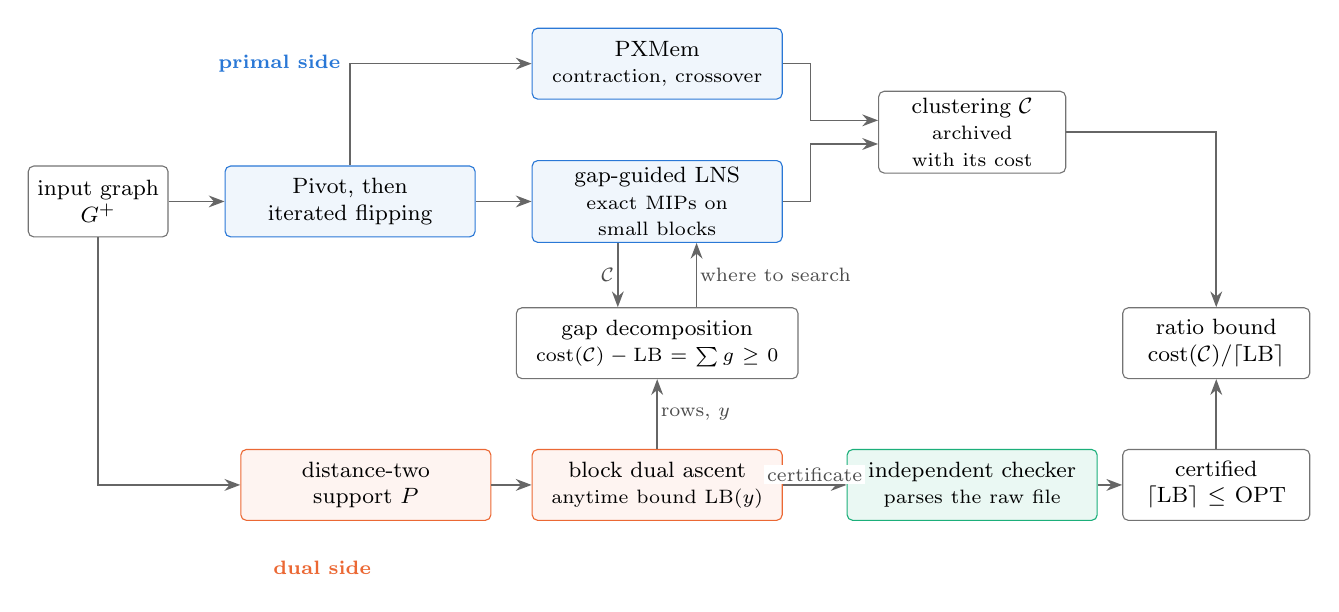
\begin{tikzpicture}[
  font=\footnotesize, >=Stealth,
  box/.style={draw=black!55, rounded corners=2pt, align=center, inner sep=2.5pt,
              minimum height=9mm, text width=30mm, fill=white},
  primal/.style={box, draw=pxblue, fill=pxblue!7},
  dual/.style={box, draw=pxorange, fill=pxorange!7},
  check/.style={box, draw=pxaqua, fill=pxaqua!9},
  outp/.style={box, text width=22mm},
  lab/.style={font=\scriptsize, text=black!70, align=center, fill=white, inner sep=1pt},
  arr/.style={->, draw=black!60, line width=0.6pt},
]
\node[box, text width=16mm] (in) at (-0.2,0) {input graph\\$G^+$};
\node[primal] (pivot) at (3.0,0) {Pivot, then\\iterated flipping};
\node[primal] (lns)   at (6.9,0) {gap-guided LNS\\\scriptsize exact MIPs on small blocks};
\node[primal] (px)    at (6.9,1.75) {PXMem\\\scriptsize contraction, crossover};
\node[outp]    (C)     at (10.9,0.88) {clustering $\mathcal C$\\\scriptsize archived with its cost};
\node[box, text width=34mm]    (gap)   at (6.9,-1.8) {gap decomposition\\\scriptsize$\cost(\mathcal C)-\LB=\sum g\ge0$};
\node[dual]   (sup)   at (3.2,-3.6) {distance-two\\support $P$};
\node[dual]   (bd)    at (6.9,-3.6) {block dual ascent\\\scriptsize anytime bound $\LB(y)$};
\node[check]  (chk)   at (10.9,-3.6) {independent checker\\\scriptsize parses the raw file};
\node[outp]    (lb)    at (14.0,-3.6) {certified\\$\lceil\LB\rceil\le\OPT$};
\node[outp]    (ratio) at (14.0,-1.8) {ratio bound\\$\cost(\mathcal C)/\lceil\LB\rceil$};

\draw[arr] (in) -- (pivot);
\draw[arr] (in.south) |- (sup.west);
\draw[arr] (pivot) -- (lns);
\draw[arr] (pivot.north) |- (px.west);
\draw[arr] (lns.east) -- ++(0.35,0) |- ([yshift=-1.5mm]C.west);
\draw[arr] (px.east) -- ++(0.35,0) |- ([yshift=1.5mm]C.west);
\draw[arr] (sup) -- (bd);
\draw[arr] (bd) -- node[lab, right] {rows, $y$} (gap);
\draw[arr] ([xshift=-5mm]lns.south) -- node[lab, left] {$\mathcal C$} ([xshift=-5mm]gap.north);
\draw[arr] ([xshift=5mm]gap.north) -- node[lab, right] {where to search} ([xshift=5mm]lns.south);
\draw[arr] (bd) -- node[lab, above] {certificate} (chk);
\draw[arr] (chk) -- (lb);
\draw[arr] (lb) -- (ratio);
\draw[arr] (C.east) -| (ratio.north);

\node[font=\scriptsize\bfseries, text=pxblue, anchor=east] at (3.0,1.75) {primal side};
\node[font=\scriptsize\bfseries, text=pxorange, anchor=west] at (1.9,-4.65) {dual side};
\end{tikzpicture}
}
\caption{Overview.  The dual side (orange) builds the distance-two support
and a lower bound by block dual ascent from a sparse star packing; the
certificate is re-checked by an independent program in exact arithmetic
against the raw instance.  The primal side (blue) computes clusterings: Pivot
and iterated flipping give a start, and either the gap-guided LNS of
CertiFlip or the memetic search PXMem improves it.  The gap decomposition
splits $\cost(\mathcal C)-\LB$ into non-negative local terms and tells the LNS
where to search.}
\label{fig:overview}
\end{figure}

\paragraph{Contributions.}
\begin{enumerate}
\item \textbf{Distance-two relaxation} (Section~\ref{sec:relax}).  Optimal
clusters have diameter at most two in $G^+$, so every pair at distance at
least three is separated in every optimal clustering.  We show that the
metric LP restricted to the pairs at distance at most two, with the triangle
inequalities through distance-three pairs kept as covering rows, is a
relaxation, and that each of its feasible points extends to a feasible point
of the full metric LP with the same cost (Theorem~\ref{thm:sparse}).  The
relaxation has $O(\sum_v\deg(v)^2)$ variables instead of $\binom n2$, and LP
rounding keeps its guarantees.  We add star and local subgraph inequalities,
which are valid for every clustering that separates the distance-three pairs.
This observation is simple; its value is that the relaxation, its dual
solutions and their certificates live on $O(\sum_v\deg(v)^2)$ pairs, which
makes checked bounds possible on graphs with $10^5$ to $10^6$ vertices.  On
such graphs, in our experiments, most of the bound comes from the star
packing on these pairs, and the LP adds to it (Section~\ref{sec:exp-cert}).

\item \textbf{Anytime block-dual bound} (Section~\ref{sec:dual}).  We compute
a lower bound by dual block-coordinate ascent: each step solves the LP of one
vertex block exactly by cutting planes, with costs equal to the current
reduced costs.  The bound is valid after every step and never decreases, and
its state is one reduced cost per pair plus the rows with positive
multipliers (Theorem~\ref{thm:anytime}).  Any packing of induced stars or bad
triangles is a feasible start.  We compute one on the sparse support by a
ruin-and-recreate local search.  This sparse star packing uses the rows of
the root bound of the KaPoCE branch-and-bound but only the pairs of the
support; where both run, it is usually weaker than the original.  On the
graphs with more than $2\cdot10^4$ vertices a long packing alone gave larger
bounds than CertiFlip's short packing followed by block LPs, at comparable
but not equal running times, and block LPs started from the long packing
raised the bound further on every graph (Sections~\ref{sec:exp-bounds}
and~\ref{sec:exp-cert}).

\item \textbf{Exactly checked certificates} (Section~\ref{sec:cert}).  A
certificate lists the rows with positive multipliers.  A checker of about
\numCheckerLines{} lines that shares no code with the solver parses the raw
instance file, verifies that it is the instance the certificate was computed
for (SHA-256 of the file and of the canonical edge list), checks the validity
of every row by enumeration or by a closed form, and evaluates the bound in
integer arithmetic.  The statement that the checker evaluates is proved in
Lean~4 (Theorem~\ref{thm:anytime}(a)).  We archive every certificate behind
every reported bound.

\item \textbf{Gap decomposition and CertiFlip} (Section~\ref{sec:gap}).  For
any clustering, the difference between its cost and the dual bound splits
exactly into non-negative terms on pairs and rows (Theorem~\ref{thm:gap}).
Re-optimising a vertex set can gain at most the gap mass that touches it,
which certifies local optimality.  CertiFlip uses the gap to choose the
neighbourhoods of a large-neighbourhood search with exact sub-MIPs, after a
flipping local search after \citet{CohenAddadLPTYZ24}, and returns a checked
bound with every solution.  We do not evaluate the gap-guided choice of
neighbourhoods separately (Appendix~\ref{app:devlog}).

\item \textbf{Computational study} (Section~\ref{sec:exp}).  On the 173
solved instances of the PACE~2021 exact track, the checked bound proves
optimality on \numPaceOptOurs{} and the root star packing of the KaPoCE
branch-and-bound on 79; averaged over instances the latter is stronger
(\numPaceMeanStar{} against \numPaceMeanOurs{} of the optimum), and the
comparison depends on density.  Our bound improves the published root
bounds of two of the 27 open instances and is below them on the others.  On
\numSnapCert{} of the \numSnapTotal{} SNAP graphs, \numSnapCertHeld{} of them
from a held-out set fixed in advance, the best checked bound of our runs
certifies the archived solutions within \numSnapGapLo{} to \numSnapGapHi{}
(median \numSnapGapMedian{}), where triangle packings leave \numBaseGapLo{}
to \numBaseGapHi{}.  The star packing supplies at least 97\% of this bound,
and block LPs started from it add a median of \numPlpGainMedian{}.  Where the
dense root bound of the KaPoCE branch-and-bound finishes (at most
$2.5\cdot10^4$ vertices), it is larger than our checked bounds on
\numRootBetter{} of \numRootN{} graphs, by up to \numRootBetterHi{}.  We compare
with the sparse star packing alone, with that root bound, and with the
metric LP on the support with triangle or star rows, so that the
contribution of each part is visible.
\end{enumerate}

A second primal solver, PXMem (Section~\ref{sec:primal}), recombines two
clusterings exactly block by block of their overlap.  We use it to measure how
tight the certificates are against strong solutions, and compare it with
KaPoCE under a protocol fixed in advance (Section~\ref{sec:exp-h2h}).  The
approximation guarantees we state for CertiFlip and PXMem, expected cost at
most $3\,\OPT$, are inherited from the Pivot start and serve only as a
safeguard; the quality of a solution is measured by its certificate.

\paragraph{Relation to certified computation.}  Certifying
algorithms~\cite{McConnellMNS11} return a witness with every output.  Safe
bounds from floating-point LP solutions~\cite{NeumaierS04safe,SteffyW13valid},
checkable certificates for mixed-integer programming~\cite{CheungGS17vipr}
and proof logging in SAT and pseudo-Boolean solving~\cite{WetzlerHH14drat,
GochtN21veripb} pursue the same goal.  Our certificates are simpler than
general MIP certificates because every row is local: its validity is decided
by enumerating the partitions of at most nine vertices or by a closed form.

\paragraph{Development and evaluation data.}  The methods were developed on
fifteen SNAP graphs and the PACE~2021 exact track.  Before the final
experiments we fixed a held-out set of twelve further SNAP graphs and the
analysis plan (Section~\ref{sec:exp-setup}).  Seven of the held-out graphs,
and the PACE heuristic-track instances, had been used once before, in an
earlier comparison with KaPoCE, run after the code had been frozen; the
heuristic-track instances that coincide with development graphs are reported
separately.
Appendix~\ref{app:devlog} records which data informed which design decision.

\section{Preliminaries and related work}\label{sec:prelim}

Let $G^+=(V,\Ep)$ with $n=|V|$ and $m=|\Ep|$; every pair not in $\Ep$ is
negative.  For a clustering $\mathcal{C}$ let $x^{\mathcal C}_{uv}=1$ if $u,v$
are in different clusters and $0$ otherwise.  Then
\[
\cost(\mathcal C)=\sum_{uv\in\Ep}x^{\mathcal C}_{uv}+\sum_{uv\notin\Ep}(1-x^{\mathcal C}_{uv}).
\]
$N(v)$ denotes the positive neighbourhood of $v$ and $d(u,v)$ the distance in
$G^+$.  The \emph{metric LP}~\cite{CharikarGW05,AilonCN08} relaxes $x$ to
$[0,1]^{\binom V2}$ subject to the triangle inequalities
$x_{uv}\le x_{uw}+x_{wv}$ for all triples.  A \emph{bad triangle} is a triple
$u,w,v$ with $uw,wv\in\Ep$ and $uv\notin\Ep$; every clustering makes at least
one mistake on it.  An \emph{induced star} with centre $v$ and $k\ge2$ leaves
is a set of $k$ pairwise non-adjacent neighbours of $v$; every clustering makes
at least $k-1$ mistakes on its $k+\binom k2$ pairs.

\paragraph{Approximation.}  Pivot repeatedly picks a uniformly random
unclustered vertex and clusters it with its unclustered positive neighbours;
its expected cost is at most three times the fractional packing LP of bad
triangles~\cite{AilonCN08}.  LP-based pivoting joins $v$ to the pivot $u$ with
probability $1-f(x_{uv})$; $f(x)=x$ gives $2.5$~\cite{AilonCN08}, and the
rounding functions of \citet{ChawlaMSY15} give $2.06$.  Both guarantees hold
against the value of \emph{any} feasible metric $x$, a fact we use below.
Further improvements use Sherali--Adams
hierarchies~\cite{CohenAddadLN22}, preclustering~\cite{CohenAddadLLN23} and
the cluster LP~\cite{CaoCLLNV24,CaoCLLLNTVYZ25,GarciaSorianoS26}; the best
combinatorial ratio, $2-2/13$, comes from a local search with
flips~\cite{CohenAddadLPTYZ24}.  For parallel, streaming, dynamic and weighted
variants see~\cite{cohenaddad2021constant,behnezhad2022almost3,DemaineEFI06}.

\paragraph{Lower bounds.}  The classical scalable bounds are packings of bad
triangles, greedy or fractional; the latter approximates the covering LP over
bad triangles and can be computed by the multiplicative-weights scheme of
Garg and K\"onemann~\cite{GargK07,Fleischer00}.  \citet{veldt2022stc} derives
LP relaxations from strong triadic closure that are supported on the open
wedges of $G^+$, like our relaxation, and yield fast $2$-approximations and
bounds within a factor of about two; our relaxation keeps the full metric LP
on these pairs and adds stronger rows.  The metric LP of correlation clustering on complete graphs has been solved
on graphs with about $10^4$ vertices by projection
methods~\cite{veldt2019metric,ruggles2020parallel}.  The Project and Forget
scheme~\cite{SonthaliaG22project}, which also keeps only active triangle
rows, reaches larger sparse instances of correlation clustering on general
graphs, where pairs without an edge carry no cost; that objective differs
from ours in the same way as the multicut objective below.  Exact branch-and-bound for cluster
editing~\cite{BockerBK11exact,BlasiusEtAl22sea} uses packings of stars and of
induced paths on three vertices as lower bounds; \citet{BlasiusEtAl22sea} mark
the pairs at distance at least three as forbidden, and \citet{BastosOPSMP16}
observe that they are separated in every optimal solution.  For the clique
partitioning problem, the weighted maximisation form, facets and cutting
planes go back to Gr\"otschel and Wakabayashi~\cite{GrotschelW89,
GrotschelW90facets}; later work removes redundant triangle
rows~\cite{MiyauchiS15redundant,miyauchi2018exact,koshimura2022concise}, adds
chorded-cycle facets~\cite{irmai2024chorded}, uses Lagrangian relaxation with
pegging tests~\cite{SukegawaYZ13lagrangian}, and tightens bounds with
constraints on subnetworks~\cite{belyi2023subnetwork}.  Exact approaches via
weighted MaxSAT~\cite{BergJ17maxsat} and kernelisation~\cite{Guo09kernel,
CaoC12kernel} solve smaller instances to optimality.

For the multicut problem on sparse graphs, where missing pairs carry no cost,
dual decomposition and message passing give fast lower
bounds~\cite{SwobodaA17multicut,AbbasS22rama,abbas2023clusterfug}, and
persistency criteria fix variables that take the same value in every optimal
solution~\cite{lange2018partial,LangeAS19persistency}.  Our block-dual ascent
is closest in spirit to block-coordinate ascent for dense graphical
models~\cite{TouraniSRS18mplp}: each block is solved to optimality with the
other multipliers fixed.  These multicut methods are not designed for correlation clustering on
complete graphs, where the $\binom n2-m$ negative pairs all carry cost, but
the distance-two support reduces the complete instance to a sparse one.  For
every clustering $\mathcal C$, the multicut objective on the graph $(V,P)$
with weight $+1$ on $\Ep$ and $-1$ on $\Nt$ counts the positive pairs between
clusters and subtracts the negative pairs of $P$ between clusters, so it
differs from $\cost(\mathcal C)$ by a constant ($|\Nt|$) plus the number of
negative pairs outside $P$ inside clusters, which is non-negative.  Hence any
multicut lower bound on $(V,P)$, plus $|\Nt|$, is a valid lower bound for
correlation clustering, and dual solvers such as RAMA~\cite{AbbasS22rama}
can be run on the support.  We ran RAMA (Table~\ref{tab:snap-lp}); the
following argument shows why such bounds cannot exceed a weak relaxation.
Dual methods based on cycle inequalities give at most the value of the
multicut LP on $(V,P)$ with all cycle inequalities.  Every feasible point of
$\mathrm{LP}_P$ extends to a metric on $V$ (Theorem~\ref{thm:sparse}(b)) and
therefore satisfies all cycle inequalities of $(V,P)$, and the two objectives
agree up to the constant $|\Nt|$.  So these bounds are at most the value of
$\mathrm{LP}_P$ with triangle rows, which on the SNAP graphs is far below our
checked bounds wherever it converged (Table~\ref{tab:snap-lp}); the RAMA
bounds are below it on every graph where it converged.

\paragraph{Heuristics.}  Local search with vertex
moves~\cite{elsner2009bounding}, Louvain and Leiden with the constant Potts
model at resolution $1/2$, which optimise the same
objective~\cite{veldt2018lambdacc,BlondelGLL08,TraagWvE19}, heuristics for
clique partitioning~\cite{BruscoK09clique,ZhouHG16threephase,LuZH22hybrid},
local search for multicut~\cite{levinkov2017comparative} and fusion
moves~\cite{BeierHK15fusion} are the common primal methods.  KaPoCE combines
reductions, local search and an evolutionary
phase~\cite{BlasiusEtAl21kapoceHeur}.  SCC~\cite{hausberger2025scc} is a
multilevel memetic solver for correlation clustering on sparse signed graphs,
in which pairs without an edge carry no cost; its objective therefore differs
from the complete-graph objective studied here (Section~\ref{sec:exp-setup}).
Twin (critical-clique) reductions and their weighted variants are standard in
parameterised algorithms and practical tools~\cite{Guo09kernel,
ProttiDS09modular,BockerBBT09weighted,Bocker12golden,ChenM12kernel,
WittkopBLR07force,WittkopEtAl10transclust}.

\section{Lower bounds on the distance-two support}\label{sec:bounds}

\subsection{Distance-two relaxations}\label{sec:relax}

\begin{lemma}\label{lem:half}
Let $\mathcal C$ be an optimal clustering, $S\in\mathcal C$ and $v\in S$.  Then
$|N(v)\cap S|\ge (|S|-1)/2$.  Consequently any two vertices of $S$ are
adjacent or have a common neighbour in $S$.  In particular every pair at
distance at least three is separated.
\end{lemma}
\begin{proof}
Moving $v$ to a singleton changes the cost by $|N(v)\cap S|-(|S|-1-|N(v)\cap
S|)$, which must be non-negative.  For non-adjacent $u,v\in S$ the sets
$N(u)\cap S$ and $N(v)\cap S$ lie in $S\setminus\{u,v\}$, which has $|S|-2$
elements, and have total size at least $|S|-1$, so they intersect.
\end{proof}

Lemma~\ref{lem:half} is folklore; its consequence for distance-three pairs is
noted by \citet{BastosOPSMP16} and used to forbid pairs in the
branch-and-bound of \citet{BlasiusEtAl22sea}.  What follows uses it to
restrict the LP rather than the search.

Let $\Nt=\{uv\notin\Ep: N(u)\cap N(v)\ne\emptyset\}$, $P=\Ep\cup\Nt$ and
$F=\binom V2\setminus P$ (the \emph{far} pairs).  Note
$|P|\le m+\sum_{w}\binom{\deg(w)}{2}$.  Figure~\ref{fig:support} shows
the support on a small neighbourhood of a collaboration network: already
there, 587 of the 780 pairs (75\%) are far and disappear from the relaxation.

\begin{figure}[!tbp]
\centering
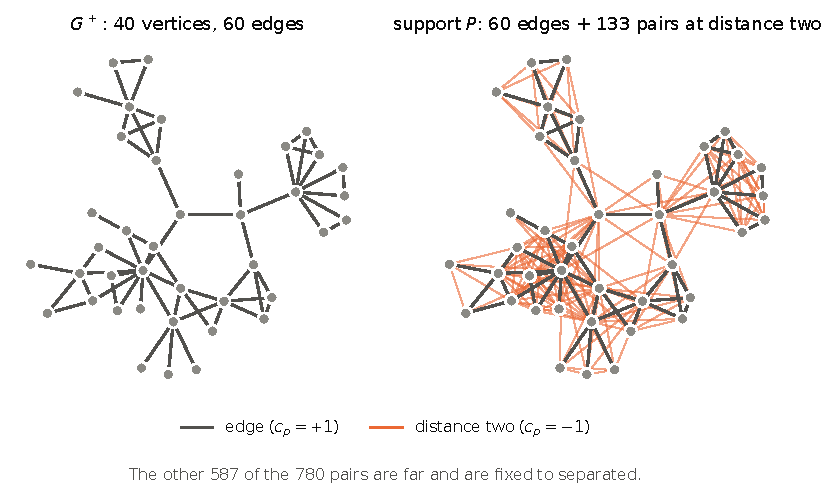
\includegraphics[width=0.9\textwidth]{figures/fig_support.pdf}
\caption{The distance-two support on a 40-vertex neighbourhood of
\texttt{ca-GrQc}.  Left: the positive graph.  Right: the support $P$ adds the
non-adjacent pairs with a common neighbour (orange); every other pair is far,
separated in every optimal clustering (Lemma~\ref{lem:half}), and carries no
variable.}\label{fig:support}
\end{figure}

\begin{definition}[distance-two relaxation]
$\mathrm{LP}_P$ has a variable $x_e\in[0,1]$ for every $e\in P$ and minimises
$\sum_{e\in\Ep}x_e+\sum_{e\in\Nt}(1-x_e)$ subject to
\begin{align}
x_{uv}&\le x_{uw}+x_{wv} &&\text{for all } u,v,w \text{ with } uv,uw,wv\in P,\label{eq:t1}\\
x_{uw}+x_{wv}&\ge 1 &&\text{for all } u,v,w \text{ with } uw,wv\in P,\ uv\in F.\label{eq:t2}
\end{align}
\end{definition}

\begin{theorem}\label{thm:sparse}
Let $\mathrm{LP}_{\mathrm{std}}$ denote the value of the metric LP.
\begin{enumerate}
\item[(a)] $\mathrm{LP}_{\mathrm{std}}\le \mathrm{LP}_P\le\OPT$.
\item[(b)] If $x$ is feasible for $\mathrm{LP}_P$, then $\bar x$, defined as $x$ on
$P$ and $1$ on $F$, is feasible for the metric LP and has the same cost.
\item[(c)] Let $\mathcal A$ be a randomised rounding algorithm with
$\mathbb E[\cost(\mathcal A(\bar x))]\le\alpha\,\mathrm{cost}(\bar x)$ for every
feasible metric $\bar x$.  Applied to an optimal solution of $\mathrm{LP}_P$ it
is an $\alpha$-approximation.  This holds in particular for $\alpha=2.5$
(ACN) and $\alpha=2.06$ (CMSY).  With pivot-based rounding, only pairs in
$P$ can be joined, so the rounding takes $O(n+|P|)$ time.
\end{enumerate}
\end{theorem}
\begin{proof}
(b) Consider a triple $u,v,w$ and the number of far pairs among $uv,uw,wv$.
With none, all three triangle inequalities are rows~\eqref{eq:t1}.  With
exactly one, say $uv$, the inequality $\bar x_{uv}=1\le x_{uw}+x_{wv}$ is
row~\eqref{eq:t2}.  The other two inequalities, such as
$x_{uw}\le 1+x_{wv}$, hold because $x\le 1$.  With two or three far pairs, each
inequality has a right-hand side of at least $1$.  Far pairs are negative and
$\bar x=1$ on them, so they contribute $0$ to the cost.  (a) The first
inequality follows from (b).  For the second, by Lemma~\ref{lem:half} an
optimal clustering separates all far pairs.  Its cut vector restricted to $P$
therefore satisfies~\eqref{eq:t1} and~\eqref{eq:t2}, because it is a metric
with $x=1$ on $F$, and it has cost $\OPT$.  (c) follows from (a) and (b): the
expected cost is at most $\alpha\,\mathrm{cost}(\bar x)=\alpha\,\mathrm{LP}_P
\le\alpha\,\OPT$.  Pivot-based rounding joins $v$ to the pivot $u$ with
probability $1-f(x_{uv})$, and $f(1)=1$ for both rounding functions.
\end{proof}

The rows~\eqref{eq:t1}--\eqref{eq:t2} are generated lazily.  A violated row
needs $x_{uw}+x_{wv}<1$, so separation around a vertex $w$ only has to look at
pairs of ``close'' neighbours in $P$, which keeps it fast in practice.

\paragraph{Stronger inequalities.}  The integrality gap of the metric LP is
at least $2$ (stars attain it asymptotically) and at most
$2.06$~\citep{ChawlaMSY15}.  We add two families that are valid for every clustering
separating all far pairs, and hence for every optimal clustering.

\begin{proposition}\label{prop:subgraph}
Let $\mathcal C$ be a clustering in which no far pair shares a cluster.
\begin{enumerate}
\item[(i)] (star inequalities; the case $|S|=1$ of the $2$-partition
inequalities of \citet{GrotschelW89}, with the far pairs dropped from the
second sum, which makes them stronger and valid only for far-separating
clusterings) For every $v$ and $T\subseteq V\setminus\{v\}$, with
$y=1-x^{\mathcal C}$,
\[\textstyle\sum_{t\in T}y_{vt}-\sum_{\{t,t'\}\subseteq T,\ tt'\in P}y_{tt'}\le 1.\]
\item[(ii)] (local subgraph inequalities) For every $H\subseteq V$,
\[\textstyle\sum_{e\in\Ep(H)}x^{\mathcal C}_e+\sum_{e\in\Nt(H)}(1-x^{\mathcal C}_e)\ \ge\ \OPT(H),\]
where $\OPT(H)$ is the optimum of the instance induced by $H$ and $\Ep(H)$,
$\Nt(H)$ are the pairs of $\Ep$ and $\Nt$ inside $H$.  More strongly, the
right-hand side may be the minimum over the clusterings of $H$ that separate
the far pairs inside $H$, which can exceed $\OPT(H)$; the checker accepts
every row with this stronger right-hand side (Section~\ref{sec:cert}).  These
are the subnetwork constraints of \citet{belyi2023subnetwork} in the
minimisation form.
\end{enumerate}
\end{proposition}
\begin{proof}
(i) If the cluster of $v$ contains $k$ vertices of $T$, the first sum is $k$
and the second is at least $\binom k2$.  Pairs inside $T$ that are not in $P$
are far, so they are separated and contribute $0$ to the second sum.
Finally $k-\binom k2\le1$.  (ii) Restricted to $H$, $\mathcal C$ is a clustering
of $H$.  Its mistakes inside $H$ number at least $\OPT(H)$.  The far pairs
inside $H$ are separated and cost nothing, so all its mistakes are counted
on the left-hand side.
\end{proof}

The local subgraph inequalities are local cuts in the sense of
\citet{ApplegateBCC01localcuts}: valid inequalities obtained by solving a small
subproblem exactly.  Bad triangles ($\OPT=1$) and induced stars with $k$ independent leaves
($\OPT=k-1$) are local subgraph inequalities.  So are chordless cycles $C_k$
with odd $k$, for which $\OPT(C_k)=\lceil k/2\rceil$ while $x=1/2$ on the
cycle edges gives $k/2$; rounding the total bound up recovers one such half
unit, the row recovers one for every cycle.  We separate stars greedily around
each vertex.  For (ii) we grow $H$ ($|H|\le 8$) by breadth-first search along
fractional pairs and compute $\OPT(H)$ by enumerating the at most $4140$
set partitions of $H$.

\subsection{Anytime dual bounds}\label{sec:dual}

Write the relaxation as $\min\{K+c^\top x: Ax\ge b,\ 0\le x\le 1\}$ over
$x\in\R^P$, with $c_e=1$ on $\Ep$, $c_e=-1$ on $\Nt$ and $K=|\Nt|$.  The rows
of $(A,b)$ are any valid inequalities from Section~\ref{sec:relax}.

\begin{theorem}\label{thm:anytime}
For every $y\ge 0$ let $r=c-A^\top y$ and
\begin{equation}\label{eq:lb}
\LB(y)=K+b^\top y+\sum_{e\in P}\min\{0,r_e\}.
\end{equation}
\begin{enumerate}
\item[(a)] $\LB(y)\le\OPT$.
\item[(b)] Let $B\subseteq V$, let $R_B$ be a set of rows supported on pairs
with both endpoints in $B$, and let $\bar r$ be the reduced costs after
removing the contribution of the current multipliers on $R_B$.  Replace these
multipliers by an optimal dual solution of
$\min\{\bar r^\top x_B: A_Bx_B\ge b_B,\ 0\le x_B\le 1\}$.  This does not
decrease $\LB$.
\item[(c)] If $B=V$ and $R_B$ consists of all rows of $\mathrm{LP}_P$
together with all rows that carry a positive multiplier, one block step gives
$\LB\ge\mathrm{LP}_P$, with equality if $R_B$ has no further rows.
\end{enumerate}
\end{theorem}
\begin{proof}
(a) Let $\mathcal C$ be optimal.  By Lemma~\ref{lem:half} it separates far
pairs, so $\OPT=K+c^\top x^{\mathcal C}$ with $x^{\mathcal C}\in\{0,1\}^P$
satisfying $Ax^{\mathcal C}\ge b$.  Then
$\OPT=K+r^\top x^{\mathcal C}+y^\top Ax^{\mathcal C}\ge K+\sum_e\min\{0,r_e\}+y^\top b$.
(b) By LP duality the block LP equals
$\max_{y_B\ge0}\ b_B^\top y_B+\sum_{e\in P_B}\min\{0,(\bar r-A_B^\top
y_B)_e\}$.  The terms of~\eqref{eq:lb} outside the block do not change, and
the old multipliers are feasible for this maximisation.  (c) With $B=V$ and
every row with a positive multiplier in $R_B$, removing their contribution
gives $\bar r=c$, so the block LP is $\mathrm{LP}_P$ with the rows of $R_B$
added, whose value is at least $\mathrm{LP}_P$ and equal to it if no row is
added; by LP duality with the box constraints, $\LB$ equals this value.  If a
row with a positive multiplier were left outside $R_B$, $\bar r\ne c$ and the
bound could be below $\mathrm{LP}_P$.
\end{proof}

Part~(b) needs an optimal block dual.  When a block LP stops at its time limit,
its duals are only feasible; the bound computed with them is still valid by
part~(a), but it may be smaller than before.  The implementation therefore
evaluates the new bound and keeps a block step only if the bound does not
decrease, so the bound is monotone in every case.

\paragraph{Warm start by star packings.}  Every pair-disjoint family of
induced stars (a centre $v$ with $k\ge2$ pairwise non-adjacent positive
neighbours) is a feasible dual solution: put $y=1$ on the corresponding
local subgraph inequalities of Proposition~\ref{prop:subgraph}(ii), which in
$x$-form read $\sum_t x_{vt}-\sum_{tt'}x_{tt'}\ge (k-1)-\binom k2$.  Then
$\LB(y)$ equals the packing value $\sum(k-1)$.  Indeed, a centre pair has
$c_e=1$ and coefficient $1$, and a leaf pair has $c_e=-1$ and coefficient
$-1$, so every packed pair has reduced cost $0$.  Unpacked pairs keep
$r_e=c_e$.  Hence $\LB=K+\sum_S\big((k_S-1)-\binom{k_S}2\big)-|\Nt\setminus
\text{packed}|$, and $K-|\Nt\setminus\text{packed}|=\sum_S\binom{k_S}{2}$.
Fractional packings of bad triangles, as computed by the Garg--K\"onemann
scheme~\citep{GargK07,Fleischer00}, are installed in the same way on the
rows $x_{uw}+x_{wv}-x_{uv}\ge0$.
Packings are the bounds used inside the KaPoCE branch-and-bound
algorithm~\citep{BlasiusEtAl22sea}.  Its implementation stores the instance
as a dense matrix, so it applies only to graphs with at most about $10^4$
vertices.  We build a greedy packing on the sparse support, processing
centres by decreasing degree, and improve it by \emph{ruin and recreate}.
(On dense instances large stars waste pairs, since a star with $k$ leaves
uses $k+\binom k2$ pairs for a value of $k-1$.  There we also try a packing
that first packs bad triangles maximally and then extends stars on free
pairs, as well as the fractional triangle packing, and install the best of
the candidates.)
Each step picks a random vertex, removes all stars centred in a random
connected region of about 12 vertices around it, and repacks the freed
pairs greedily in a random order.  A step is kept iff the value does not
decrease.  The packing is installed as the initial multipliers.  Subsequent
block steps release the packed rows that lie inside a block and re-optimise
them fractionally together with newly separated rows.  By
Theorem~\ref{thm:anytime}(b), the final bound is never below the packing
value.

The bound~\eqref{eq:lb} needs only the vector $r$ and the scalar $b^\top y$.
We store the rows with positive multipliers so that a later block containing
them can re-optimise them.  Blocks of the same partition are independent.
In a \emph{sweep} we compute a partition into parts of about $2500$ vertices
with METIS~\citep{KarypisK98} on a randomly relabelled copy of $G^+$, so that
successive sweeps cut different pairs.  Each part is solved with the dual
simplex method of HiGHS~\citep{HuangfuH18}, with lazily separated triangle,
star and local subgraph rows.  After the sweeps stall we switch to
\emph{gap-guided blocks}, grown around the vertices with the largest share of
the gap of Section~\ref{sec:gap}.  Because~\eqref{eq:lb} is valid for any $y\ge0$, the
bound remains correct even when a block LP hits its time limit.  We only
clamp the dual values to be non-negative, and reject a block step that would
lower the bound.

\paragraph{Floating point.}  The block LPs are solved in double precision,
so the multipliers $y$ are inexact and the rows they carry are generated by
floating-point separation.  Neither affects validity: \eqref{eq:lb} holds for
every $y\ge0$ and every set of valid rows.  The value the solver reports is
nevertheless not the value we publish.  Section~\ref{sec:cert} recomputes it
from the exported rows and multipliers in exact arithmetic, after checking
every row, and all bounds in Section~\ref{sec:exp} are these recomputed
values.


\section{Certificates and their independent check}\label{sec:cert}

Every lower bound reported in Section~\ref{sec:exp} is the output of a
separate checker, not of the solver.  This section specifies what a
certificate contains, what the checker verifies, and what has to be trusted.

\paragraph{Contents.}  A certificate is a compressed NumPy archive with
\begin{itemize}
\item the rows with positive multiplier, in compressed sparse row form: for
row $i$ the pairs $p=\{u,v\}$ of its support, integer coefficients $a_{ip}$
and an integer right-hand side $b_i$, in the $x$-form $a_i^\top x\ge b_i$;
\item the multipliers $y_i\ge0$ as double-precision numbers;
\item the identity of the instance: the name and relative path of the raw file
as distributed by PACE or SNAP, its SHA-256, its format, the number of
vertices $n$ and edges $m$, and the SHA-256 of the canonical edge list, that
is, of $n$ followed by the lexicographically sorted pairs $(u,v)$ with $u<v$
as 64-bit integers.
\end{itemize}
The vertex numbering is fixed by the instance definition: a PACE file numbers
the vertices $1,\dots,n$; in a SNAP edge list the vertices are the identifiers
that occur in a kept edge, numbered in increasing order, a signed list keeps
only its positive rows, and self-loops and duplicate edges are dropped.  The
clustering whose cost is reported is archived next to the certificate, one
label per vertex in the same numbering.

\paragraph{The check.}  The checker (\texttt{experiments/check\_certificate.py},
\numCheckerLines{} lines of Python with Numba kernels) imports nothing from
the solver package.  Given the raw file and the certificate it
\begin{enumerate}
\item parses the raw file with its own reader and rejects the certificate
unless it records $n$, $m$, the file hash and the edge-list hash and all four
agree with the file.  When it checks a directory, the instance file named in a
certificate must be listed with the same hash in the committed manifest of
instance files, and the parser settings of that file (format and sign column)
are taken from a committed instance table, never from the certificate, so a
certificate can neither choose the instance it is checked against nor how
that instance is read;
\item checks the shape, type, length and range of every array before
converting it: one-dimensional arrays, integer vertex ids in $[0,n)$ and
offsets, real and finite coefficients, right-hand sides and multipliers, and
equal lengths of the arrays that describe the same entries or rows;
\item checks that every pair of every row is in $P$, i.e.\ is an edge or has a
common neighbour, by intersecting sorted adjacency lists;
\item checks that no row contains a pair twice and that the absolute values
of the coefficients of every row sum to less than $2^{61}$, so that every
partial sum below is exact in 64-bit integers;
\item checks that every row is valid for every clustering that separates the
far pairs.  A row on at most nine vertices is checked by enumerating all
partitions of its vertex set (at most $21{,}147$, as restricted growth
strings) that separate its far pairs and taking the minimum of the integer
left-hand side.  A larger row is accepted only if it is a star row: its
positive entries are the pairs $vt$, $t\in T$, of one centre $v$, and its
negative entries are pairs $R$ inside $T$.  Its minimum over far-separating
clusterings is at least $|T|-|R|-M$ with $M=1$ if $R$ contains every non-far
pair inside $T$ (then a far-free subset of $T$ is a clique of $R$) and $M$
the independence number of $(T,R)$ otherwise, computed exactly.  (If $K\subseteq
T$ is the set of leaves in the cluster of $v$ and $e_R(K)$ the number of pairs
of $R$ inside $K$, the left-hand side is at least $|T|-|R|-(|K|-e_R(K))$.  In
the first case $K$ is a clique of $R$ and $|K|-\binom{|K|}2\le1$; in the
second, $|K|-e_R(K)$ is at most the number of connected components of
$(K,R)$, since a component with $s$ vertices has at least $s-1$ edges, and
hence at most the independence number of $(T,R)$.)
\item rounds each $y_i$ down to a multiple of $2^{-30}$ and evaluates
\begin{equation}\label{eq:checked}
\LB=\sum_i b_iy_i+\sum_{p\in P}\Bigl(\min\bigl\{0,\,c_p-\textstyle\sum_i a_{ip}y_i\bigr\}-\min\{0,c_p\}\Bigr)
\end{equation}
in integer arithmetic (64-bit accumulation under a checked overflow bound,
then arbitrary-precision integers), and returns $\lceil\LB\rceil$;
\item optionally evaluates the cost of the archived clustering on the parsed
instance, also in integers.
\end{enumerate}
Rounding down keeps $y\ge0$, so the rounded multipliers are again a dual
certificate; nothing else in~\eqref{eq:checked} is inexact.  The sum runs
over the pairs that occur in some row, since the other terms vanish.
Expression~\eqref{eq:checked} is~\eqref{eq:lb} with $K=|\Nt|=
-\sum_{p\in P}\min\{0,c_p\}$ absorbed.

\begin{proposition}\label{prop:checker}
If the checker accepts a certificate for an instance, then the value it
returns is at most $\OPT$ of that instance.
\end{proposition}
\begin{proof}
By steps 3 and 5, every row is supported on $P$ and satisfied by the cut
vector of every clustering that separates far pairs.  By
Lemma~\ref{lem:half} this includes every optimal clustering, and
Theorem~\ref{thm:anytime}(a) with the rounded multipliers gives $\LB\le\OPT$.
$\OPT$ is an integer.
\end{proof}

The inequality behind the proof, that~\eqref{eq:checked} is at most the cost
of every far-separating clustering for any rows valid for such clusterings,
is proved in Lean~4 (\texttt{far\_dual\_bound}, \texttt{far\_dual\_le\_opt};
Appendix~\ref{app:lean}), as is the fact that optimal clusterings separate far
pairs; row validity is a hypothesis there.  The procedures that decide it
(steps 3--5), the reader and the integer evaluation are tested, not verified,
and so is the closed form for star rows with an incomplete $R$, whose
validity argument is the one given in step~5; no archived certificate uses
that case.  What remains to be trusted is therefore the checker's reader, the
enumeration and the star formula of step~5, the integer evaluation, and the
Python, NumPy and Numba (LLVM) runtime; running the checker with
\texttt{NUMBA\_DISABLE\_JIT=1} removes the compiled kernels from this list
at the price of speed (Section~\ref{sec:exp-time}).  Every archived certificate records the edge
hash computed by the solver's loader, so the acceptance of all of them shows
that the two readers agree on every instance we use.  The tests of the
repository check the star formula against the enumeration on random star
rows with at most nine vertices, the integer cost of a clustering against the
solver's, and the rejection of certificates with a perturbed right-hand side,
a negative or out-of-range multiplier, a pair outside $P$, a missing instance
hash or a different instance.  An earlier version of the checker converted
the multipliers to 64-bit integers before checking their range, so a
certificate with a multiplier above $2^{33}$ would have wrapped around to a
negative value and been accepted with a wrong bound.  This was found in
review and fixed; the largest multiplier in any archived certificate is \numMaxY{}.
A second review found that the enumeration summed the coefficients of a row
in 64-bit integers without a bound on the row, so a row that repeats one pair
thousands of times with coefficients near $2^{51}$ wrapped around and was
accepted as valid; step~4 now rejects such rows (the largest sum of absolute
coefficients of a row in any archived certificate is \numMaxRowAbs{}).  A third
review found that the checker did not compare the lengths of the arrays, so
a certificate whose coefficient array was shorter than its pair arrays was
not rejected, and that it accepted complex coefficients; step~2 now rejects
both, and non-finite values explicitly.  All three cases are regression
tests, and all archived certificates were re-checked with the final version
(Section~\ref{sec:exp-time}).

\paragraph{Relation to proof formats.}  VIPR~\cite{CheungGS17vipr} certifies
a mixed-integer program by a derivation: cutting planes and branching
disjunctions, each checked syntactically.  A local row of ours would need a
branching derivation over all far-separating partitions of its vertices, up
to $21{,}147$ leaves per row, so we decide its validity semantically by
enumerating these partitions instead, which enlarges the trusted base by the
enumeration code but keeps a certificate to the rows and their multipliers.
Proof logging for pseudo-Boolean and constraint
solvers~\cite{GochtN21veripb,GochtMMNPT20} certifies combinatorial bounds of
the same local kind through cutting-plane derivations, with verified checkers
available; translating our rows into such a format would give a second,
independent check and is left open.  The certificate format is specified,
independently of the checker's code, in
\texttt{docs/certificate\_format.md}, including the byte layout of the edge
hash and the reading rules for PACE and SNAP files, so that other solvers can
write certificates; the checker accepts the packings of the KaPoCE
branch-and-bound exported in this format (Section~\ref{sec:exp-cert}).  In
single-file use the parser settings are read from the certificate unless
given on the command line, and are printed as part of the result; only the
directory mode of step~1 takes them from the committed instance table.

\paragraph{Cost of checking.}  Checking is much cheaper than computing the
bound: the largest certificate we report, on \texttt{\numCheckMaxGraph}, has
\numCheckMaxRows{} rows, and no archived certificate takes more than
\numRecheckMax{}\,s to check, including reading the instance
(Section~\ref{sec:exp-time}).  One command re-checks every archived
certificate against freshly downloaded instance files and writes one line per
certificate.

\paragraph{What is not certified.}  The certificate proves a lower bound, and
the archived clustering an upper bound; together they bound the gap of the
reported solution.  The approximation guarantees of Theorems~\ref{thm:sparse}
and~\ref{thm:certiflip} are statements about the algorithms, not about a
particular run, and are not checked.  Running times are measured, not
certified.

\section{Gap decomposition and CertiFlip}\label{sec:gap}

A dual solution does more than bound the optimum: together with a clustering
it says where the clustering can still improve.  This section makes that
precise and uses it in a primal method that returns a certificate with every
solution.


\begin{theorem}\label{thm:gap}
Let $y\ge0$, $r=c-A^\top y$, and let $\mathcal C$ be a clustering that separates all
far pairs.  Then
\begin{equation}\label{eq:gap}
\cost(\mathcal C)-\LB(y)=\sum_{e\in P}\underbrace{\big(r_ex^{\mathcal C}_e-\min\{0,r_e\}\big)}_{g_e\ge0}
+\sum_i\underbrace{y_i\,(a_i^\top x^{\mathcal C}-b_i)}_{s_i\ge0}.
\end{equation}
\end{theorem}
\begin{proof}
$\cost(\mathcal C)=K+c^\top x^{\mathcal C}=K+r^\top x^{\mathcal C}+y^\top
Ax^{\mathcal C}$.  Subtract~\eqref{eq:lb}.  Each $g_e\ge0$ because
$x_e\in\{0,1\}$, and each $s_i\ge0$ by the validity of row $i$.
\end{proof}

A pair term vanishes iff the clustering agrees with the sign of the reduced
cost.  A row term vanishes iff the row is tight or has multiplier $0$.
Assigning each term to the endpoints of its pairs gives a \emph{gap map} over
the vertices.

\begin{corollary}[local certificate]\label{cor:local}
For $B\subseteq V$ let $\Gamma_B(\mathcal C)$ be the sum of the terms
of~\eqref{eq:gap} whose pair, or one of whose row pairs, has an endpoint in
$B$.  Let $\mathcal C'$ be any clustering that separates far pairs and
coincides with $\mathcal C$ on all pairs with both endpoints outside $B$.  Then
$\cost(\mathcal C)-\cost(\mathcal C')\le\Gamma_B(\mathcal C)$.  In particular,
if $\Gamma_B(\mathcal C)<1$ then no re-clustering of $B$ improves $\mathcal C$.
\end{corollary}
\begin{proof}
Apply~\eqref{eq:gap} to both clusterings.  Terms not touching $B$ coincide,
and the terms of $\mathcal C'$ are non-negative.  Costs are integers.
\end{proof}

\paragraph{Gap-guided LNS.}  Large-neighbourhood search~\citep{Shaw98}, here
with exact sub-MIPs in the spirit of RINS and local
branching~\citep{DannaRL05rins,FischettiL03local}, fixes
the clustering outside a vertex set $B$ ($|B|\le 60$) and re-optimises $B$
exactly.  Let $\mathcal K$ be the outside clusters with a positive edge into
$B$.  Re-clusterings of $B$ correspond to clusterings of $B$ together with one
super node per $K\in\mathcal K$, where super nodes must stay apart.  The cost is
$\sum_{uv}[uv\in\Ep]x_{uv}+[uv\notin\Ep](1-x_{uv})$ for $u,v\in B$, plus
$w_{vK}x_{vK}+(|K|-w_{vK})(1-x_{vK})$ for each $v\in B$, where $w_{vK}$ counts
the positive edges between $v$ and $K$.  We solve this MIP with HiGHS and add
triangle inequalities lazily until the solution is transitive.  To keep
Corollary~\ref{cor:local} applicable, $v$ may join $K$ only if it is within
distance two of every member of $K$, and far pairs inside $B$ are fixed apart.
Neighbourhoods are grown around high-gap vertices, either by breadth-first
search or as a union of whole clusters.  Neighbourhoods with $\Gamma_B<1$ are
skipped because they are certified optimal.  Theorem~\ref{thm:gap} and
Corollary~\ref{cor:local} need a clustering that separates far pairs, which
the output of the flipping search need not do.  Before the search, and after
every improvement, we therefore move to a singleton every vertex $v$ with
$|N(v)\cap S|<(|S|-1)/2$ in its cluster $S$, until there is none.  Each such
move lowers the cost, and by the argument of Lemma~\ref{lem:half} the result
separates all far pairs.  The certificate $\Gamma_B<1$ covers re-clusterings
of $B$ that also separate far pairs; by Lemma~\ref{lem:half} these include
every optimal one.

Figure~\ref{fig:gapmap} shows the gap map at work on the neighbourhood of
Figure~\ref{fig:support}.  For a Pivot clustering the gap of 10 is
concentrated on one cluster; the LNS re-optimises the blocks around the
high-gap vertices and reaches a clustering whose cost equals the bound, which
certifies it optimal.

\begin{figure}[!tbp]
\centering
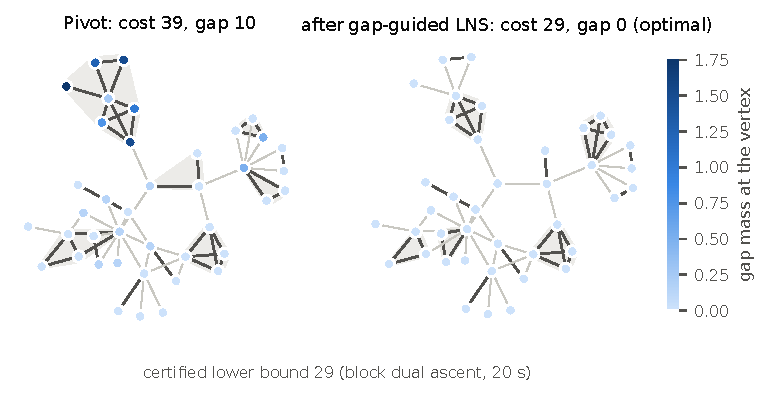
\includegraphics[width=0.92\textwidth]{figures/fig_gapmap.pdf}
\caption{Gap decomposition (Theorem~\ref{thm:gap}) on the neighbourhood of
Figure~\ref{fig:support}.  Each vertex is coloured by its share of
$\cost(\mathcal C)-\LB$ (pair terms split between the endpoints, row terms
between the vertices of the row); shaded regions are clusters, dark edges lie
inside a cluster.  Left: a Pivot clustering.  Right: after gap-guided LNS the
gap is zero, so the clustering is optimal.  Computed by the released code.}
\label{fig:gapmap}
\end{figure}


\subsection{CertiFlip}\label{sec:algo}

\begin{algorithm}[t]
\caption{CertiFlip$(G^+,T)$}\label{alg:certiflip}
\begin{algorithmic}[1]
\State $\mathcal C\gets\textsc{Pivot}(G^+)$ with a uniformly random order
\State $\mathcal C\gets\textsc{IteratedFlip}(\mathcal C)$ \Comment{insertion local search with flips}
\State build the distance-two support $P$
\State $y\gets$ star packing with ruin-and-recreate local search \Comment{feasible dual}
\State $y\gets\textsc{BlockAscent}(P,y,\mathcal C)$ \Comment{METIS sweeps, then gap-guided blocks}
\If{one block covered $V$ and separation converged}
  \State $\mathcal C\gets$ best of $\mathcal C$ and \textsc{IteratedFlip}(\textsc{CMSY-Round}$(x^\star)$) over several roundings
\EndIf
\State $\mathcal C\gets\textsc{GapLNS}(\mathcal C,y)$ until time $T$
\State \Return $\mathcal C$ and $\lceil\LB(y)\rceil$ \Comment{lines 4--5 target half of the remaining budget}
\end{algorithmic}
\end{algorithm}

\paragraph{Insertion local search.}  For every root $r$ we build one candidate
insertion $S(r)$ by \emph{cleaning} $N[r]$.  Starting from $S=N[r]$, we
repeat a few sweeps over $v\in N[r]\setminus\{r\}$: we put $v$ in $S$ iff
joining $S$ costs $v$ less than staying in the remainder of its current
cluster.  Both costs are computed exactly from counts of weighted positive
neighbours.  We then compute the exact change of the objective in
$O(\sum_{v\in S}\deg v)$ time and apply the insertion if it is negative.
Rounds of insertions alternate with a multilevel (Louvain-type) vertex-move
local search.  That search works on the weighted objective, moves super nodes
at coarse levels and hence also merges clusters.  \textsc{IteratedFlip}
follows \citet{CohenAddadLPTYZ24}.  Positive weights take values in
$\{1,1.5,2\}$ (we double all weights to stay in integers).  Each round flips
the pairs cut by the previous solution, re-optimises, flips and re-optimises
again, and combines the last three solutions with their $3$-way pivot.  The
best candidate under the original objective is returned.

\begin{theorem}\label{thm:certiflip}
Let $\mathcal C$ and $\LB$ be the output of Algorithm~\ref{alg:certiflip}.
\begin{enumerate}
\item[(a)] $\mathbb E[\cost(\mathcal C)]\le3\,\OPT$.
\item[(b)] $\LB\le\OPT$, so $\cost(\mathcal C)/\lceil\LB\rceil$ is an upper
bound on the approximation ratio achieved on the instance.
\item[(c)] If line~7 is executed, $\mathbb E[\cost(\mathcal C)]\le 2.06\,\OPT$.
\end{enumerate}
\end{theorem}
\begin{proof}
Every step after line~1 returns a clustering no worse than its input: the
local searches only apply improving moves, \textsc{IteratedFlip} returns the
best of its candidates, which include the local optimum reached from its input,
and \textsc{GapLNS} accepts only improvements.  (a) then follows from the
Pivot guarantee~\citep{AilonCN08}.  (b) is Theorem~\ref{thm:anytime}(a) and
the integrality of $\OPT$.  (c) If one block covered $V$ and separation
converged, the block LP primal $x^\star$ satisfies all
rows~\eqref{eq:t1}--\eqref{eq:t2}, so it is feasible for $\mathrm{LP}_P$.
A block covering $V$ contains every row with a positive multiplier (packed
rows are released into it), so its costs are the original costs $c$
(Theorem~\ref{thm:anytime}(c)) and the cost of $x^\star$ is the value of the
block LP.  Every row of the block LP is valid for an
optimal clustering (Lemma~\ref{lem:half} and Proposition~\ref{prop:subgraph}),
whose cut vector is therefore feasible for the block LP; hence the block LP
value is at most $\OPT$.  By Theorem~\ref{thm:sparse}(b,c),
$\mathbb E[\cost(\textsc{CMSY-Round}(x^\star))]\le 2.06\,\OPT$.  The remaining
steps are monotone.  (The LP solver returns $x^\star$ in floating point and
feasible up to its tolerance; part~(c) is a statement about the exact
optimum, unlike part~(b), which is checked exactly.)
\end{proof}

\begin{remark}
Part~(a) holds for any procedure that starts from a Pivot clustering and never
makes its solution worse; it is a safeguard, not a distinguishing property.
If the insertion local search reached an optimum with respect to
\emph{all} cluster insertions, \citet{CohenAddadLPTYZ24} would give a factor of
$2$, and $2-2/13$ with enough flipping rounds.  Our candidate generation
explores a polynomial subfamily of insertions, so we do not claim these
factors.  The certificate of Theorem~\ref{thm:certiflip}(b), however, is
valid in every case.
\end{remark}

\paragraph{Running time.}  Pivot takes $O(n+m)$ time.  One round of insertions
takes $O(\sum_v\sum_{u\in N(v)}\deg u)=O(\sum_u\deg(u)^2)$, the same order as
the size of $P$ and the number of bad triangles.  The support takes
$O(\sum_w\deg(w)^2)$ time and memory.  The block LPs dominate the running
time, and the time spent on them is set by the budget $T$.


\paragraph{Budget.}  The budget $T$ is checked between steps: before each
block LP, each LNS neighbourhood and each flipping round.  A single round of
the insertion local search, the construction of the support and a sub-MIP
are not interrupted, so a run can exceed $T$.  Section~\ref{sec:exp} reports
the measured wall-clock and CPU times of every run, including these overruns,
and the time at which the final bound was reached.

\section{Computational study}\label{sec:exp}

\subsection{Setup}\label{sec:exp-setup}

\paragraph{Implementation and machines.}  All methods are implemented in
Python with Numba-compiled kernels (package \texttt{ccbench}).  LPs and MIPs
are solved with HiGHS~1.15~\cite{HuangfuH18} and graph partitions are
computed with METIS~\cite{KarypisK98}.  The runs of CertiFlip, of the
star packings, of the metric LP on $P$ and of the head-to-head
comparison were made on Google Colab virtual machines with two logical cores
and \SI{12.7}{GB} of memory, one run per machine at a time, with the CPU model
recorded in every result file (\numCpuModels; the AMD model on
\numCpuAmd{}, the Intel model on all others).  The triangle packings, three of the
KaPoCE root bounds on SNAP graphs, the rerun of its root bounds on the PACE
exact track, SCC and the rows marked $^a$ in
Table~\ref{tab:pace-primal} were run on 4-core workstations with several runs
in parallel; these are marked where they appear.  The \SI{1800}{s} bound
runs and the triangle LPs on every fourth PACE exact instance
(Section~\ref{sec:exp-bounds}) were run on a laptop (\numCpuLocal), and RAMA
on a laptop GPU.  Every run uses one thread.
Budgets are wall-clock times; CPU times are recorded as well.

\paragraph{Instances.}  Table~\ref{tab:instances} lists the SNAP
graphs~\cite{LeskovecK14snap}, used as complete instances with $\Ep$ given by
the edges (for signed networks, by the positive
edges~\cite{leskovec2010signedchi,kumar2016bitcoin}).  Fifteen of them were
used during development; the twelve held-out graphs were chosen afterwards to
span $10^3$ to $10^6$ vertices and several graph classes.  They were fixed
before any bound was computed on them and before any run of the protocol
below; seven of them are also PACE heuristic-track instances and had been run
once, in an earlier comparison of the two solvers made after the code was
frozen (Appendix~\ref{app:devlog}).  We also use the 200
instances of each track of PACE~2021~\cite{KellerhalsKNZ21pace}: the exact
track ($n\le620$; 173 instances with known optimum and 27 open) and the
heuristic track (up to $2\cdot10^6$ vertices).  Ten heuristic-track instances
coincide with development graphs and seven with held-out graphs
(Table~\ref{tab:instances}).

\begin{table}[!tbp]
\centering
\caption{SNAP instances: vertices, edges, size of the distance-two support
$P$ and role.  ``--'': the estimate $m+\sum_v\binom{\deg v}2$ of the support
exceeds $3\cdot10^7$ pairs, a threshold fixed in advance from the memory of
the machines; CertiFlip and the block LPs were not run on these graphs, the
star packings were (Table~\ref{tab:snap-bounds}); $^\ast$: $|P|$ as measured
by the ruin-and-recreate packing, which builds the support.  PACE: the
heuristic-track instance with the same graph.}
\label{tab:instances}
\small
\begin{adjustbox}{max width=\textwidth}\begin{tabular}{lrrrll}
\toprule
graph & $n$ & $m$ & $|P|$ & role & PACE \\
\midrule
\texttt{ca-GrQc} & \num{5242} & \num{14484} & \num{78224} & dev & heur167 \\
\texttt{ca-HepTh} & \num{9877} & \num{25973} & \num{205421} & dev & heur173 \\
\texttt{ca-HepPh} & \num{12008} & \num{118489} & \num{1638915} & dev & heur175 \\
\texttt{ca-AstroPh} & \num{18772} & \num{198050} & \num{4639091} & dev & heur176 \\
\texttt{ca-CondMat} & \num{23133} & \num{93439} & \num{1169993} & dev & heur178 \\
\texttt{email-Enron} & \num{36692} & \num{183831} & \num{15241801} & dev & heur179 \\
\texttt{loc-Brightkite} & \num{58228} & \num{214078} & \num{8576618} & dev &  \\
\texttt{soc-Epinions} & \num{75879} & \num{405740} & \num{36788203}$^\ast$ & dev & heur180 \\
\texttt{Slashdot+} & \num{75144} & \num{382882} & \num{35019657}$^\ast$ & dev &  \\
\texttt{Epinions+} & \num{114467} & \num{592591} & \num{56948607}$^\ast$ & dev &  \\
\texttt{BitcoinOTC+} & \num{5573} & \num{18591} & \num{972669} & dev &  \\
\texttt{BitcoinAlpha+} & \num{3683} & \num{12972} & \num{493107} & dev &  \\
\texttt{com-Amazon} & \num{334863} & \num{925872} & \num{6933597} & dev & heur193 \\
\texttt{com-DBLP} & \num{317080} & \num{1049866} & \num{13718957} & dev & heur191 \\
\texttt{com-Youtube} & \num{1134890} & \num{2987624} & -- & dev & heur198 \\
\midrule
\texttt{email-Eu-core} & \num{1005} & \num{16064} & \num{223665} & held-out & heur094 \\
\texttt{facebook} & \num{4039} & \num{88234} & \num{1446301} & held-out & heur166 \\
\texttt{wiki-Vote} & \num{7115} & \num{100762} & \num{3473778} & held-out &  \\
\texttt{cit-HepTh} & \num{27770} & \num{352285} & \num{15155045}$^\ast$ & held-out &  \\
\texttt{cit-HepPh} & \num{34546} & \num{420877} & \num{11577385} & held-out &  \\
\texttt{p2p-Gnutella31} & \num{62586} & \num{147892} & \num{1663263} & held-out &  \\
\texttt{soc-Slashdot0902} & \num{82168} & \num{504230} & \num{49698358}$^\ast$ & held-out & heur186 \\
\texttt{loc-Gowalla} & \num{196591} & \num{950327} & -- & held-out & heur188 \\
\texttt{email-EuAll} & \num{265214} & \num{364481} & -- & held-out &  \\
\texttt{amazon0302} & \num{262111} & \num{899792} & \num{6588959} & held-out & heur189 \\
\texttt{web-NotreDame} & \num{325729} & \num{1090108} & -- & held-out & heur192 \\
\texttt{roadNet-PA} & \num{1088092} & \num{1541898} & \num{4421718} & held-out & heur197 \\
\bottomrule
\end{tabular}
\end{adjustbox}
\end{table}

\paragraph{Lower bounds compared.}  All bounds are rounded up to integers.
Bounds marked \emph{checked} are values returned by the checker of
Section~\ref{sec:cert} from an archived certificate.
\begin{itemize}
\item \emph{Triangle packings}: a maximal pair-disjoint packing of bad
triangles (the bound of MatchFlipPivot~\cite{veldt2022stc}) and a
fractional packing by the Garg--K\"onemann scheme with
$\varepsilon=0.05$~\cite{GargK07,Fleischer00}, scaled by its maximum load.
\item \emph{Star local search} (SLS, checked): the star-packing local search
of Section~\ref{sec:dual}, compiled C++ (\texttt{experiments/sstar},
\texttt{g++ -O2}), for \SI{600}{s} on the SNAP graphs and \SI{60}{s} on the
PACE exact track, the budget of the CertiFlip runs there, with seeds 0--4;
seed~0 is reported unless stated otherwise.  It runs until the time limit,
as a minimum time; the certificate is written from its stars without
building the support.  On \texttt{com-Youtube} and \texttt{email-EuAll} a
star has at most 100 leaves.  Controls: with the stopping rule of the KaPoCE
branch-and-bound and \SI{60}{s} only as a cap (PACE exact, seeds 0--4; the
rule counts rounds, so these runs were made partly on a 4-core cloud machine
with a \SI{2.8}{GHz} Xeon, three at a time); \SI{300}{s} on the PACE
instances closed only by the CertiFlip bound; \SI{1200}{s} on the SNAP graphs
with a support; and \SI{3600}{s} on the SNAP graphs on which it did not
approach its stopping rule within \SI{600}{s}.
\item \emph{SLS, then block LPs} (SLS+LP, checked): the star local search for
\SI{600}{s}, then METIS block sweeps from its packing for \SI{600}{s}, on the
SNAP graphs with a support.
\item \emph{Ruin-and-recreate star packing} (R\&R, checked): the greedy star
packing on $P$ improved by ruin and recreate, installed as a dual solution
without any LP.
The number of iterations is set before the run from the iteration rate
measured on the instance, so as to fill the budget; the measured running
times, which can be well above it, are reported.
\item \emph{Metric LP on $P$}: $\mathrm{LP}_P$ with triangle
rows~\eqref{eq:t1}--\eqref{eq:t2} only, solved by cutting planes with HiGHS
until no row is violated or the budget ends; and the same with star rows.
These are LP values in floating point, reported to separate the strength of
the relaxation from the dual method.
\item \emph{CertiFlip bound} (checked): Theorem~\ref{thm:anytime}, as
computed within CertiFlip, whose bound phase targets half of the remaining
budget but does not interrupt a block LP (measured times in
Section~\ref{sec:exp-time}), and, on a subset of PACE instances, with a long
budget and one block covering the graph.
\item \emph{R\&R, then block LPs} (R\&R+LP, checked): the ruin-and-recreate
packing with half of a \SI{1200}{s} budget, followed by METIS block sweeps
from it for the other half, as one procedure; by
Theorem~\ref{thm:anytime}(b) the result is never below the packing it starts
from.  One run per graph (seed~0) on the SNAP graphs with a support.
\item \emph{RAMA}: the multicut dual of \citet{AbbasS22rama} (commit
\texttt{ee459d6}, GPU solver, lower bound only) on the support $P$ with weight
$+1$ on $\Ep$ and $-1$ on $\Nt$, plus $|\Nt|$ (Section~\ref{sec:prelim});
run on a laptop GPU (NVIDIA RTX A2000).  RAMA prints its bound with six
significant digits, and the values are not certified.
\item \emph{KaPoCE root bounds}: the star-packing and $P_3$-packing bounds of
the KaPoCE branch-and-bound~\cite{BlasiusEtAl22sea}.  On the PACE exact track
we use the values published by its authors, and check them against a rerun
without data reductions (Section~\ref{sec:exp-bounds}); these are not
certified.  On the SNAP graphs with at most
$2.5\cdot10^4$ vertices we ran its lower-bound program (branch \texttt{experiments}, commit
\texttt{63079a9}, four-hour limit, one run per graph; three graphs on a
4-core workstation, the others on the 2-core Colab machines) ourselves; its
dense matrices do not fit into memory on the larger graphs.  On these graphs
we also exported its final star packing and checked it as a certificate
(Section~\ref{sec:exp-cert}).
\end{itemize}

\paragraph{Solvers compared.}  Pivot~\cite{AilonCN08}, the best of 50
Pivot runs, MatchFlipPivot~\cite{veldt2022stc}, vertex-move local
search~\cite{elsner2009bounding}, our multilevel Louvain-type local search,
Leiden with the constant Potts model at resolution
$1/2$~\cite{TraagWvE19,veldt2018lambdacc}, our iterated flipping local search,
CertiFlip, PXMem, and KaPoCE~\cite{BlasiusEtAl21kapoceHeur}, the winner of both
PACE~2021 tracks (heuristic version, commit \texttt{\numKapoceCommit}).  SCC~\cite{hausberger2025scc}
optimises the objective of sparse signed graphs, in which a pair without an
edge costs nothing, whereas here every non-edge is a negative pair.  We run it
(commit \texttt{05d0849}, memetic version with one process) on the complete
encoding, in which every non-adjacent pair is an explicit edge of weight
$-1$.  This needs $\binom n2$ edges and is feasible on the PACE exact track
(Section~\ref{sec:exp-bounds}) but not on the SNAP graphs.

\subsection{Lower bounds on the PACE exact track}\label{sec:exp-bounds}

\begin{table}[!tbp]
\centering
\caption{PACE~2021 exact track, the 173 instances with known optimum: lower
bounds.  Checked (values returned by the checker from archived
certificates): the ruin-and-recreate star packing, the CertiFlip bound
(budget \SI{60}{s}; measured times in Section~\ref{sec:exp-time}), the
CertiFlip bound with \SI{1800}{s} (every fourth instance), the star local
search (\SI{60}{s}) and the larger of the CertiFlip bound and the star local
search.  Not certified: the triangle
packings, computed earlier on a 4-core workstation; the metric LP on $P$, a
floating-point LP value reported only where cutting planes converged within
\SI{900}{s} (every fourth instance); the two B\&B rows, the root bounds of the
KaPoCE branch-and-bound as published by its authors (reproduced by a rerun
without data reductions, see the text); and the last row, which
takes the larger of a checked and a published value.}
\label{tab:pace-bounds}
\footnotesize
\begin{tabular}{lrrrr}
\toprule
bound & instances & mean LB/OPT & min LB/OPT & LB $=$ OPT \\
\midrule
greedy triangle packing & 173 & 0.8612 & 0.660 & 14 \\
fractional triangle packing & 173 & 0.9664 & 0.811 & 30 \\
ruin-and-recreate star packing & 173 & 0.8712 & 0.247 & 17 \\
CertiFlip bound & 173 & 0.9874 & 0.816 & 106 \\
CertiFlip bound, 1800 s & 45 & 0.9948 & 0.940 & 34 \\
star local search & 173 & 0.9984 & 0.960 & 122 \\
metric LP on $P$, triangle rows & 39 & 0.9762 & 0.814 & 21 \\
B\&B star packing~\cite{BlasiusEtAl22sea} & 173 & 0.9948 & 0.891 & 79 \\
B\&B $P_3$ packing~\cite{BlasiusEtAl22sea} & 173 & 0.9742 & 0.813 & 59 \\
larger of CertiFlip and star local search & 173 & 0.9989 & 0.972 & 130 \\
larger of both and B\&B star & 173 & 0.9989 & 0.972 & 131 \\
\bottomrule
\end{tabular}

\end{table}

\begin{table}[!tbp]
\centering
\caption{Mean LB/OPT on the solved PACE exact instances by edge density
$m/\binom n2$.  The fractional triangle packing was computed earlier on a
4-core workstation.}
\label{tab:pace-density}
\footnotesize
\setlength{\tabcolsep}{4pt}
\begin{tabular}{lrrrrr}
\toprule
edge density & instances & CertiFlip & sparse star & fractional & B\&B star \\
 & & bound & packing & triangle packing & packing \\
\midrule
$[0,0.1)$ & 35 & 0.9978 & 0.9529 & 0.9614 & 0.9934 \\
$[0.1,0.3)$ & 40 & 0.9781 & 0.8623 & 0.9646 & 0.9971 \\
$[0.3,0.5)$ & 48 & 0.9823 & 0.9046 & 0.9448 & 0.9914 \\
$[0.5,1)$ & 50 & 0.9923 & 0.7892 & 0.9922 & 0.9974 \\
\bottomrule
\end{tabular}

\end{table}

\paragraph{Strength of the bounds.}  The star local search, run for
\SI{60}{s} per instance, gives the strongest bound on this track
(Table~\ref{tab:pace-bounds}).  Its mean LB/OPT on the 173 solved instances
is \numPaceSlsMean{}, against \numPaceMeanStar{} for the root star packing of
the KaPoCE branch-and-bound as published and \numPaceMeanOurs{} for the
CertiFlip bound, and it is at least \numPaceSlsMin{} of the optimum on every
instance.  It proves optimality on \numPaceSlsOpt{} instances, against 79 for
the B\&B star packing, 59 for its $P_3$ packing and \numPaceOptOurs{} for the
CertiFlip bound, and together with the CertiFlip bound, both checked, on
\numPaceBestOpt{} (mean \numPaceBestMean{}).  Against the published B\&B star
packing it is larger on \numPaceSlsAbove{} instances, equal on
\numPaceSlsEqual{} and smaller on \numPaceSlsBelow{}; adding that bound to
the two checked ones proves optimality on only one more instance
(\numPaceBestMaxOpt{}).  The advantage holds in every density band
(Table~\ref{tab:pace-density}).  The CertiFlip bound is larger than the star
local search on \numPaceSlsUnderCf{} instances, by one to eight units, and
proves optimality on eight of them, where the star local search does not:
there the block LPs close the last units.  Below density $0.1$ the two are
equal on average.  Each run took about the budget (median \numPaceSlsTimeMedian{}\,s,
at most \numPaceSlsTimeMax{}\,s, including the certificate).

All three star packings pack the same induced stars, and our earlier
ruin-and-recreate packing reaches only \numPacePackMean{} on average
(Table~\ref{tab:pace-bounds}): the difference lies in the packing
heuristic.  The published data state neither the time
spent on the root bounds nor whether they were computed after the data
reductions of the branch-and-bound, so we reran its lower-bound program on
the input graphs, without reductions (the program of
Section~\ref{sec:exp-cert}, \SI{900}{s} limit, one run per instance;
\numKrootPaceColab{} on the Colab machines, one at a time, the others on a
4-core cloud machine with a \SI{2.2}{GHz} Xeon, at most three at a time).
The star packing finished within the limit on \numKrootPaceStarN{} of the
\numKrootPaceN{} instances (\numKrootPaceTimeoutList{} stopped after the $P_3$
packing).  Its $P_3$ packing equals the published value on
\numKrootPacePthreeEqual{} of \numKrootPacePthreeN{}, its star packing on
\numKrootPaceStarEqual{}, and on the others the star packing differs by at
most \numKrootPaceStarDiffMax{} (\numKrootPaceStarAbove{} larger,
\numKrootPaceStarBelow{} smaller, at most \numKrootPaceStarRelMax{}; the
heuristic uses a random generator, which we ran with its default seed, and
the published values may come from another version).  The star bound took a
median of \numKrootPaceTimeMedian{}\,s and at most \numKrootPaceTimeMax{}\,s.
The published root bounds are therefore bounds of the input graphs.  The
heuristic stops by its own rule, after five times as many rounds as improved
the packing; the star local search instead runs until its time limit.

On every fourth instance we also ran the bound with \SI{1800}{s} and one
block covering the graph, and the metric LP on $P$ with triangle rows only.
With the longer budget the mean LB/OPT on these \numPaceWarmN{} instances is
\numPaceWarmMean{}, against \numPaceWarmOursMean{} with the \SI{60}{s} runs
and \numPaceWarmStarMean{} for the B\&B star packing, and the bound is
optimal on \numPaceWarmOpt{} of them (\numPaceWarmOursOpt{} at \SI{60}{s}).
The triangle LP converged within \SI{900}{s} on \numPaceTriN{} of these
instances, with a mean LB/OPT of \numPaceTriMean{} (\numPaceTriOursMean{}
for our bound on the same instances).  Of the \numWarmRuns{} bound runs,
\numWarmLocal{} were made on a laptop (\numCpuLocal), several at a time, and one
on a Colab machine.  The limit applies to the LP phase; the star-packing warm
start before it (sized to about 30\% of the limit) and the certificate come
on top, and \numWarmOver{} of the \numWarmRuns{} runs took longer than
\SI{1800}{s}, the longest \numWarmMax{}\,s.  The checker accepted all their
certificates.

\paragraph{Open instances.}  Of the \numPaceOpen{} instances of the exact
track without a known optimum, our best checked bound exceeds the larger
published root bound~\cite{BlasiusEtAl22sea} on \numPaceOpenImproved{}
(Table~\ref{tab:pace-open}); on \texttt{exact179} it leaves a gap of one to
the best known solution.  On the other \numPaceOpenBelow{} it is smaller than
the published root bound, by at most \numPaceOpenMaxBelow{}.  None of the
open instances is closed.

\begin{table}[!tbp]
\centering
\caption{Open instances of the PACE~2021 exact track on which the checked
lower bound improves the published one.  Published bounds: the best upper
bound and the larger of the two root bounds of~\cite{BlasiusEtAl22sea}; our
UB: the CertiFlip run of Table~\ref{tab:pace-bounds}; checked LB: the largest
checked bound of our runs.}
\label{tab:pace-open}
\footnotesize
\begin{tabular}{lrrrrrr}
\toprule
instance & $n$ & $m$ & published UB & published LB & our UB & checked LB \\
\midrule
\texttt{exact042} & 100 & 1563 & \num{1055} & \num{1006} & \num{1055} & \num{1017} \\
\texttt{exact043} & 100 & 1624 & \num{984} & \num{968} & \num{984} & \num{978} \\
\texttt{exact051} & 120 & 2251 & \num{1619} & \num{1508} & \num{1619} & \num{1533} \\
\texttt{exact052} & 120 & 2448 & \num{1473} & \num{1431} & \num{1473} & \num{1442} \\
\texttt{exact060} & 124 & 2288 & \num{1491} & \num{1427} & \num{1491} & \num{1446} \\
\texttt{exact069} & 140 & 2915 & \num{2140} & \num{1994} & \num{2140} & \num{2015} \\
\texttt{exact070} & 140 & 3014 & \num{1792} & \num{1762} & \num{1792} & \num{1779} \\
\texttt{exact082} & 160 & 4015 & \num{2434} & \num{2397} & \num{2434} & \num{2414} \\
\texttt{exact083} & 160 & 4259 & \num{2939} & \num{2808} & \num{2941} & \num{2824} \\
\texttt{exact091} & 180 & 4602 & \num{3234} & \num{3072} & \num{3236} & \num{3087} \\
\texttt{exact092} & 180 & 6067 & \num{3563} & \num{3520} & \num{3563} & \num{3529} \\
\texttt{exact101} & 200 & 6731 & \num{4198} & \num{4135} & \num{4198} & \num{4148} \\
\texttt{exact102} & 200 & 6746 & \num{3925} & \num{3895} & \num{3925} & \num{3903} \\
\texttt{exact103} & 200 & 7081 & \num{4572} & \num{4381} & \num{4572} & \num{4382} \\
\texttt{exact105} & 200 & 12309 & \num{5320} & \num{5314} & \num{5320} & \num{5318} \\
\texttt{exact179} & 330 & 1370 & \num{633} & \num{620} & \num{633} & \num{632} \\
\texttt{exact180} & 330 & 2256 & \num{1081} & \num{1052} & \num{1083} & \num{1073} \\
\texttt{exact181} & 330 & 3253 & \num{1563} & \num{1513} & \num{1568} & \num{1532} \\
\texttt{exact182} & 330 & 4329 & \num{2159} & \num{2091} & \num{2165} & \num{2100} \\
\texttt{exact183} & 330 & 5613 & \num{2789} & \num{2717} & \num{2788} & \num{2735} \\
\texttt{exact184} & 330 & 7270 & \num{3684} & \num{3582} & \num{3692} & \num{3597} \\
\texttt{exact195} & 620 & 3992 & \num{2529} & \num{2450} & \num{2533} & \num{2476} \\
\bottomrule
\end{tabular}

\end{table}

\begin{table}[!tbp]
\centering
\caption{PACE~2021 exact track (200 instances): primal quality against the
best known value (published upper bound or better value of any run).
CertiFlip: the certificate runs of Table~\ref{tab:pace-bounds}, one seed on
the Colab machines; SCC: one seed on the complete encoding, on a 4-core
machine with three runs in parallel; $^a$: best of three seeds from earlier
runs on the same 4-core machine with four runs in parallel.}
\label{tab:pace-primal}
\footnotesize
\begin{tabular}{lrrr}
\toprule
method & best known & mean gap (\%) & max gap (\%) \\
\midrule
CertiFlip (60 s) & 192/200 & 0.006 & 0.32 \\
SCC~\cite{hausberger2025scc} (60 s) & 200/200 & 0.000 & 0.00 \\
KaPoCE (60 s)$^a$ & 200/200 & 0.000 & 0.00 \\
IteratedFlip$^a$ & 187/200 & 0.007 & 0.32 \\
Leiden-CPM$^a$ & 158/200 & 0.119 & 3.00 \\
Pivot$^a$ & 13/200 & 32.635 & 229.54 \\
\bottomrule
\end{tabular}

\end{table}

\paragraph{Primal quality.}  On the exact track the primal side is not the
bottleneck (Table~\ref{tab:pace-primal}).  CertiFlip finds the best known
value on \numCfHit{} of the 200 instances although it spends a large part
of its \SI{60}{s} on the bound; SCC on the complete encoding and KaPoCE find it
on all of them.  The certified gaps on this track are therefore determined by
the bound.


\subsection{Certified gaps on SNAP graphs}\label{sec:exp-cert}

\begin{table}[!tbp]
\centering
\caption{SNAP graphs: checked lower bounds and certified gaps.  UB: the
best archived clustering (re-checked from its file; -- if none was archived).
CertiFlip: the best checked bound of three CertiFlip runs of \SI{600}{s}
(seeds 0--2), with the median time of their bound phase; packing: the
checked bound of one run of the sparse star packing alone (seed~0), with its
running time; pack.+LP: one run of the long packing followed by block LPs
(\SI{1200}{s}, seed~0); the largest is in bold.  Rows with -- for CertiFlip:
support above the threshold of Table~\ref{tab:instances}, packing only.  B\&B
root: the root star-packing bound of the KaPoCE branch-and-bound, run on
graphs with at most $2.5\cdot10^4$ vertices, not certified, $^\dagger$ where
it exceeds all checked bounds.  gap: $(\mathrm{UB}-\LB)/\LB$ with the largest
checked bound; gap$^*$: the same with the best value of any run of any solver
(reported, not archived); tri.\ factor: best known value divided by the
better of the two triangle packings.  Upper block: development graphs; lower
block: held-out graphs.}
\label{tab:snap-bounds}
\footnotesize
\setlength{\tabcolsep}{2.5pt}
\begin{tabular}{lrrrrrrrrrrr}
\toprule
graph & UB & \multicolumn{5}{c}{checked LB, one run each} & best & B\&B & gap & gap$^*$ & tri.\\
\cmidrule(lr){3-7}
 & & CertiFlip & R\&R & R\&R & SLS & SLS & checked & root & (\%) & (\%) & factor \\
 & & & packing & +LP & & +LP & LB & & & & \\
\midrule
\texttt{ca-GrQc} & \num{6051} & \num{6036} & \num{6003} & \num{6034} & \num{6029} & \textbf{\num{6038}} & \num{6038} & \num{6015} & 0.22 & 0.20 & 1.28 \\
\texttt{ca-HepTh} & \num{15861} & \num{15682} & \num{15705} & \textbf{\num{15725}} & \num{15697} & \num{15706} & \num{15730}$^\S$ & \num{15670} & 0.83 & 0.53 & 1.45 \\
\texttt{ca-HepPh} & \num{46194} & \num{43199} & \num{42865} & \num{43740} & \num{45969} & \textbf{\num{45974}} & \num{46001}$^\ddagger$ & \num{46014}$^\dagger$ & 0.42 & 0.29 & 1.17 \\
\texttt{ca-AstroPh} & \num{125682} & \num{118224} & \num{117865} & \num{119101} & \num{123935} & \textbf{\num{123955}} & \num{124381}$^\ddagger$ & t.o. & 1.05 & 0.93 & 1.46 \\
\texttt{ca-CondMat} & \num{56974} & \num{55283} & \num{55627} & \num{55910} & \textbf{\num{56420}} & \num{56417} & \num{56478}$^\ddagger$ & mem. & 0.88 & 0.63 & 1.43 \\
\texttt{email-Enron} & \num{150701} & \num{140551} & \num{140854} & \num{140862} & \textbf{\num{144207}} & \num{144166} & \num{144804}$^\ddagger$ & -- & 4.07 & 3.88 & 1.77 \\
\texttt{loc-Brightkite} & \num{175081} & \num{163366} & \num{163927} & \num{164106} & \textbf{\num{169694}} & \num{169661} & \num{170553}$^\ddagger$ & -- & 2.65 & 2.43 & 1.71 \\
\texttt{soc-Epinions} & -- & -- & \num{344995} & -- & \textbf{\num{349706}} & -- & \num{350862}$^\ddagger$ & -- & -- & 4.07 & -- \\
\texttt{Slashdot+} & -- & -- & \num{334298} & -- & \textbf{\num{336751}} & -- & \num{339024}$^\ddagger$ & -- & -- & 3.78 & -- \\
\texttt{Epinions+} & -- & -- & \num{489582} & -- & \textbf{\num{498929}} & -- & \num{500570}$^\ddagger$ & -- & -- & 4.24 & -- \\
\texttt{BitcoinOTC+} & \num{16497} & \num{15582} & \num{15642} & \num{15661} & \num{15909} & \textbf{\num{15911}} & \num{15937}$^\ddagger$ & \num{15927} & 3.51 & 3.29 & 1.80 \\
\texttt{BitcoinAlpha+} & \num{11461} & \num{10749} & \num{10802} & \num{10820} & \num{11061} & \textbf{\num{11062}} & \num{11088}$^\ddagger$ & \num{11038} & 3.36 & 3.15 & 1.81 \\
\texttt{com-Amazon} & \num{615035} & \num{562505} & \num{574956} & \num{576376} & \textbf{\num{594310}} & \num{593290} & \num{596984}$^\ddagger$ & -- & 3.02 & 2.57 & 1.43 \\
\texttt{com-DBLP} & \num{608183} & \num{582821} & \num{589979} & \num{589275} & \textbf{\num{600982}} & \num{600373} & \num{602651}$^\ddagger$ & -- & 0.92 & 0.68 & 1.42 \\
\texttt{com-Youtube} & -- & -- & -- & -- & \textbf{\num{2516213}}$^k$ & -- & \num{2516213} & -- & -- & 5.29 & -- \\
\midrule
\texttt{email-Eu-core} & \num{12732} & \num{11657} & \num{11413} & \num{11651} & \textbf{\num{12251}} & \num{12227} & \num{12282}$^\ddagger$ & \num{12228} & 3.66 & 3.66 & 1.59 \\
\texttt{facebook} & \num{53547} & \num{43344} & \num{42953} & \num{44025} & \num{52330} & \textbf{\num{52347}} & \num{52518}$^\ddagger$ & \num{52739}$^\dagger$ & 1.96 & 1.96 & 1.37 \\
\texttt{wiki-Vote} & \num{95263} & \num{85487} & \num{85522} & \num{85548} & \num{87595} & \textbf{\num{87600}} & \num{87743}$^\ddagger$ & t.o. & 8.57 & 8.57 & 1.90 \\
\texttt{cit-HepTh} & \num{293167} & -- & \num{266019} & -- & \textbf{\num{277208}} & -- & \num{280009}$^\ddagger$ & -- & 4.70 & 4.70 & -- \\
\texttt{cit-HepPh} & \num{357463} & \num{322666} & \num{324327} & \num{324608} & \textbf{\num{336163}} & \num{336120} & \num{339821}$^\ddagger$ & -- & 5.19 & 5.18 & 1.72 \\
\texttt{p2p-Gnutella31} & \num{131362} & \num{130297} & \textbf{\num{130336}} & \num{130326} & \num{130020} & \num{130010} & \num{130546}$^\S$ & -- & 0.63 & 0.63 & 1.79 \\
\texttt{soc-Slashdot0902} & \num{470778} & -- & \num{447216} & -- & \textbf{\num{449403}} & -- & \num{453147}$^\ddagger$ & -- & 3.89 & 3.88 & -- \\
\texttt{loc-Gowalla} & \num{788550} & -- & -- & -- & \textbf{\num{750395}} & -- & \num{757280}$^\ddagger$ & -- & 4.13 & 4.12 & -- \\
\texttt{email-EuAll} & \num{342709} & -- & -- & -- & \textbf{\num{321593}}$^k$ & -- & \num{329275}$^\ddagger$ & -- & 4.08 & 4.08 & -- \\
\texttt{amazon0302} & \num{540844} & \num{503032} & \num{511221} & \num{508994} & \textbf{\num{531655}} & \num{531166} & \num{534122}$^\ddagger$ & -- & 1.26 & 1.26 & 1.32 \\
\texttt{web-NotreDame} & \num{733709} & -- & -- & -- & \textbf{\num{576001}} & -- & \num{607100}$^\ddagger$ & -- & 20.85 & 20.85 & -- \\
\texttt{roadNet-PA} & \num{944542} & \num{865131} & \num{884166} & \num{905670} & \num{891590} & \textbf{\num{915741}} & \num{915741} & -- & 3.15 & 3.14 & 1.30 \\
\bottomrule
\end{tabular}

\end{table}

\begin{table}[!tbp]
\centering
\caption{The metric LP restricted to $P$, solved by cutting planes with HiGHS
on one core (budget \SI{1800}{s} with triangle rows and \SI{3600}{s} with
star rows, \SI{7200}{s} on \texttt{ca-GrQc}), against the best checked bound
of Table~\ref{tab:snap-bounds}, and the multicut dual bound of RAMA on the
same support plus $|\Nt|$ (Section~\ref{sec:prelim}; on one GPU, failed: the
solver stopped with a CUDA memory error).  LP and RAMA values are in floating
point and not certified.  A value in parentheses is that of the last LP when the budget
ended during its solution; it is not the optimum of any relaxation and not a
bound.  killed: the job was killed with its machine three times, most likely
for lack of memory; n.r.: not run.}
\label{tab:snap-lp}
\footnotesize
\setlength{\tabcolsep}{4pt}
\begin{tabular}{lrrrrrrrr}
\toprule
graph & best & best checked & \multicolumn{2}{c}{LP$_P$, triangle rows} & \multicolumn{2}{c}{LP$_P$, + star rows} & \multicolumn{2}{c}{RAMA} \\
\cmidrule(lr){4-5}\cmidrule(lr){6-7}\cmidrule(lr){8-9}
 & known & LB & value & time (s) & value & time (s) & value & time (s) \\
\midrule
\texttt{ca-GrQc} & \num{6050} & \num{6038} & \num{4931} & 2 & \num{6039} & 2578 & \num{3944} & 30 \\
\texttt{ca-HepTh} & \num{15813} & \num{15730} & \num{11477} & 6 & (\num{14449}) & 3621 & \num{8625} & 2 \\
\texttt{ca-HepPh} & \num{46133} & \num{46001} & (\num{36932}) & 1808 & n.r. &  & \num{-4} & 3 \\
\texttt{ca-AstroPh} & \num{125541} & \num{124167} & (\num{73161}) & 1821 & n.r. &  & failed &  \\
\texttt{ca-CondMat} & \num{56834} & \num{56478} & \num{41820} & 797 & n.r. &  & \num{24394} & 319 \\
\texttt{email-Enron} & \num{150419} & \num{144804} & killed &  & n.r. &  & \num{-30} & 11 \\
\texttt{loc-Brightkite} & \num{174695} & \num{170553} & killed &  & n.r. &  & failed &  \\
\texttt{BitcoinOTC+} & \num{16462} & \num{15937} & \num{9262} & 34 & (\num{11312}) & 3605 & \num{0} & 4 \\
\texttt{BitcoinAlpha+} & \num{11437} & \num{11088} & \num{6475} & 19 & (\num{8434}) & 3604 & \num{2737} & 444 \\
\texttt{com-Amazon} & \num{612307} & \num{596984} & killed &  & n.r. &  & \num{362915} & 257 \\
\texttt{com-DBLP} & \num{606723} & \num{601440} & killed &  & n.r. &  & failed &  \\
\texttt{email-Eu-core} & \num{12732} & \num{12282} & \num{8032} & 207 & (\num{8523}) & 3618 & failed &  \\
\texttt{facebook} & \num{53547} & \num{52518} & (\num{21639}) & 1805 & (\num{43700}) & 3610 & \num{-3} & 147 \\
\texttt{wiki-Vote} & \num{95259} & \num{87743} & killed &  & n.r. &  & \num{-4} & 4 \\
\texttt{cit-HepPh} & \num{357413} & \num{339821} & killed &  & n.r. &  & \num{8} & 747 \\
\texttt{p2p-Gnutella31} & \num{131362} & \num{130546} & \num{73941} & 67 & n.r. &  & \num{71311} & 3 \\
\texttt{amazon0302} & \num{540839} & \num{534122} & (\num{429905}) & 1825 & n.r. &  & \num{326517} & 144 \\
\texttt{roadNet-PA} & \num{944519} & \num{915741} & \num{769127} & 831 & n.r. &  & \num{730910} & 5 \\
\bottomrule
\end{tabular}

\end{table}

\paragraph{Certified gaps.}  On the \numSnapCert{} of the \numSnapTotal{}
graphs whose support fits into memory, the largest checked bound
certifies the archived clusterings within \numSnapGapLo{} to \numSnapGapHi{}
(median \numSnapGapMedian{}; Table~\ref{tab:snap-bounds}).  This is the best
certificate of five runs of three procedures; taken separately, CertiFlip at
its median seed gives a median gap of \numSnapGapCfMedian{} and the packing
alone \numSnapGapPkMedian{}.  The triangle packings, the lower bounds used at
this scale so far, leave gaps of \numBaseGapLo{} to \numBaseGapHi{} on the
same graphs, the regime of the MatchFlipPivot guarantee, and the new bound is
larger on every graph.  Across the three CertiFlip seeds the bound varies by
at most \numSnapSpreadMax{}.  The largest gaps are on the held-out social and
citation graphs \texttt{facebook}, \texttt{email-Eu-core}, \texttt{wiki-Vote}
and \texttt{cit-HepPh}; the column gap$^*$ shows that no solver we ran closes
them from above, so they are due to the lower bound, the upper bound, or
both, and we cannot tell which.  The median gap is \numSnapGapMedDev{} on the
development graphs and \numSnapGapMedHeld{} on the held-out graphs.  We
attribute the difference mainly to the composition of the held-out set, which
contains the denser social and citation networks, but with seven held-out
graphs we cannot exclude that the method is tuned to the development graphs.
The other nine graphs, five of them held out, are excluded from these
statistics by a threshold on the estimated support that was fixed in
advance, not by an observed failure.  Neither the star packing nor the
checker needs the block LPs, and after the runs above we ran the packing
alone on these graphs without the threshold, on the Colab machines with
about \SI{12}{GB} of memory.  It gave checked bounds on \numPackOnlyN{} of
them (\numPackOnlyList{}; up to \numPackOnlyMaxN{} vertices, at most
\numPackOnlyTimeMax{}\,s), within \numPackOnlyGapLo{} to \numPackOnlyGapHi{}
of the best known values; on three of them no clustering was archived, so
only this gap$^*$ is given.  On the other \numNoBoundN{} (\numNoBoundList{})
the job was killed with its machine three times, most likely because our
implementation of the packing materialises the support.

\paragraph{Star packing against the block LPs.}  The sparse star packing
alone gives a larger checked bound than the CertiFlip bound on
\numPackBetter{} of the \numSnapCert{} graphs, among them all
\numPackAllAboveCount{} graphs with at least \numPackAllAbove{} vertices.
The CertiFlip bound is larger only on \numCfBetterList{}, which have at most
\numCfBetterMaxN{} vertices and are the denser ones (on \texttt{ca-AstroPh}
only as the best of three seeds; one seed is below the packing).  The two
procedures did not have the same running time
(Table~\ref{tab:snap-bounds}): the packing run took a median of
\numPackTimeMedian{}\,s (\numPackTimeLo{} to \numPackTimeHi{}\,s) and the
bound phase of CertiFlip a median of \numCfLbTimeMedian{}\,s.  On
\numPackLonger{} of the graphs where the packing wins, \numPackLongerList{},
the packing ran longer than the bound phase of every CertiFlip seed; on the
others it ran shorter.  Within CertiFlip the packing phase is short, and on large sparse graphs the
block LPs, started from a weaker packing, do not make up the difference in
the remaining time.

\paragraph{A long packing, then block LPs.}  Running the packing first with
half of a \SI{1200}{s} budget and the block LPs from it with the other half
(measured median \numPlpTimeMedian{}\,s, at most \numPlpTimeMax{}\,s; column
pack.+LP) separates the two effects.  The block LPs raised the bound above
the packing they started from on all \numPlpGainPos{} of the \numPlpN{} graphs,
by a median of \numPlpGainMedian{} and by up to \numPlpGainMax{} on
\numPlpGainMaxGraph{}, and the combined procedure gives the largest checked
bound on \numPlpBetter{} of the \numPlpN{} graphs.  On the other
\numPlpBelow{} it is below the best of the other runs by at most
\numPlpBelowMax{}: on \texttt{ca-GrQc} and \texttt{email-Eu-core} below
CertiFlip by 2 and 6, and on \texttt{com-DBLP}, \texttt{p2p-Gnutella31} and
\texttt{amazon0302} below the separate packing run, because its own packing
phase ended lower (the number of packing iterations is set from a rate
measured at the start of each run, and the two runs differ in it).  With a
strong packing as the start, the block LPs therefore add to the bound on
every graph; on the large sparse graphs what the CertiFlip bound lacks is
time for the packing, not the LP part.

\paragraph{The root bound of the branch-and-bound.}  Where it runs, on
\numRootN{} graphs with at most $2.5\cdot10^4$ vertices, the root
star-packing bound of the KaPoCE branch-and-bound exceeds all of our checked
bounds on \numRootBetterList{} (Table~\ref{tab:snap-bounds}).  As on the PACE
instances, the packing heuristic of the branch-and-bound is stronger than our
sparse one where both run; what the support adds is that a packing, and a
checked certificate for it, can be computed on graphs where the dense
implementation does not fit into memory.

\paragraph{Strength of the relaxation.}  Table~\ref{tab:snap-lp} separates
the strength of the relaxation from the way it is solved.  On
\texttt{ca-GrQc} the metric LP on $P$ with triangle rows converges in
\numGrqcTriTime{}\,s to \numGrqcTri{}, \numGrqcTriBelow{} below the best
known value (which is \numGrqcTriGap{} above it).  With star rows the LP reaches \numGrqcStar{}, \numGrqcStarGap{} below
the best known value and slightly above the best checked bound
(\numGrqcBest{}), after \numGrqcStarTime{}\,s.  The triangle inequalities,
which is what the classical metric LP has, are therefore far from sufficient
on this graph; the star inequalities close almost all of the gap, and the
anytime dual reaches nearly the same value in a tenth of the time.
RAMA, a dual method for the multicut LP with cycle inequalities, stays below
$\mathrm{LP}_P$ with triangle rows on every graph where that converged, as
the argument of Section~\ref{sec:prelim} predicts.  Its bound is at most
\numRamaFracMax{} of the best checked bound (on \numRamaFracMaxGraph{}), and on
the \numRamaNearZero{} graphs where the negative pairs dominate the support
(\numRamaNearZeroList{}) it is zero up to its printing precision.  It stopped
with an error on \numRamaFailed{} graphs.


\subsection{Running times and checking}\label{sec:exp-time}

The budgets are not hard limits (Section~\ref{sec:gap}, paragraph Budget).
Of the \numOverPaceRuns{} CertiFlip runs on the PACE exact track with
$T=\SI{60}{s}$, \numOverPaceCount{} took more than $1.01\,T$; the median
wall-clock time was \numOverPaceMedian{}\,s and the maximum
\numOverPaceMax{}\,s.  Of the \numOverSnapRuns{} runs on SNAP graphs with
$T=\SI{600}{s}$, \numOverSnapCount{} took more than $1.01\,T$ (median
\numOverSnapMedian{}\,s, maximum \numOverSnapMax{}\,s).  Of these,
\numOverPaceLarge{} PACE runs and \numOverSnapLarge{} SNAP runs exceeded
$1.2\,T$.  The bound phase of CertiFlip targets half of the remaining budget
but does not interrupt a block LP.  On the PACE exact track it took a median
of \numLbPaceMedian{}\,s and more than \SI{30}{s} on \numLbPaceOver{} of the
\numLbPaceRuns{} runs (maximum \numLbPaceMax{}\,s); on the SNAP graphs a
median of \numLbSnapMedian{}\,s and more than \SI{300}{s} on \numLbSnapOver{}
of \numLbSnapRuns{} runs (maximum \numLbSnapMax{}\,s, on
\texttt{email-Enron}).  The LP-rounding start (line~7 of
Algorithm~\ref{alg:certiflip}) was executed on \numLpSeedPace{} of the PACE
runs and improved the clustering on \numLpSeedPaceImproved{} of them; it was
never executed on the SNAP graphs.  The large overruns come from steps that
are not interrupted: single block LPs on \texttt{email-Enron}, and on the three
PACE instances with 620 vertices and $9\cdot10^4$ to $2\cdot10^5$ edges the
bound phase and, on two of them, the LP-rounding start with the local search
after it (up to \SI{277}{s} on \texttt{exact199}).  The star local search
checks its time limit between stars and took a median of
\numSlsTimeMedian{}\,s (at most \numSlsTimeMax{}\,s) on the SNAP graphs and
\numPaceSlsTimeMedian{}\,s (at most \numPaceSlsTimeMax{}\,s) on the PACE
exact track, including its certificate.  The ruin-and-recreate packing
fixes its number of iterations in advance from a measured rate; on the SNAP
graphs (nominal \SI{600}{s}) it took \numPackTimeLo{} to \numPackTimeHi{}\,s,
and on the PACE exact track (nominal \SI{60}{s}) a median of
\numPackPaceMedian{}\,s, more than \SI{60}{s} on \numPackPaceOver{} of
\numPackPaceRuns{} runs and at most \numPackPaceMax{}\,s.  The long packing
followed by block LPs (nominal \SI{1200}{s}) took a median of
\numPlpTimeMedian{}\,s and more than \SI{1260}{s} on \numPlpTimeOver{} graphs
(at most \numPlpTimeMax{}\,s).  All times are in
the archived result files.  The
comparisons of different bound procedures in Sections~\ref{sec:exp-bounds}
and~\ref{sec:exp-cert} are therefore at comparable, not equal, running
times, except for the controls of the star local search, which compare it
under the same stopping rule or the same budget; the head-to-head comparison
of Appendix~\ref{sec:exp-h2h} is at equal elapsed time by construction.

The checker accepted all \numCertPaceOk{} certificates of the PACE runs, all
\numCertSnapOk{} of the CertiFlip runs on SNAP graphs and all
\numCertPackOk{} of the star-packing runs when they were written, and
rejected none.  After the review of the checker (Section~\ref{sec:cert}) we
re-checked all \numRecheckCerts{} archived certificates, including those of
the runs made after the review, and \numRecheckLabels{} archived clusterings
with its final version (commit \texttt{\numCheckerCommit}) against freshly
downloaded instance files whose hashes are looked up in the committed
manifest and whose parser settings are taken from the committed instance
table: \numRecheckOk{} of the \numRecheckN{} were accepted, every accepted
bound equals the one checked during its run, the slowest took
\numRecheckMax{}\,s and all together \numRecheckTotal{}\,h
(\texttt{results/mpc/recheck.csv} and \texttt{recheck\_local.csv}).  The
largest certificate, on \texttt{\numCheckMaxGraph}, has \numCheckMaxRows{}
rows.  No accepted certificate uses the independence-number case of the
star formula (\numAlphaRows{} rows), and the largest multiplier is
\numMaxY{}.  Run without its compiled kernels
(\texttt{NUMBA\_DISABLE\_JIT=1}), the checker accepted \numNojitN{}
certificates, every fifth star local search and every tenth CertiFlip
certificate of the PACE exact track and two on \texttt{ca-GrQc}, with the
same values.

\section{Conclusion}\label{sec:concl}

Lower bounds that scale to large correlation clustering instances, packings
of bad triangles, certify only factors of about two.  On sparse graphs, three
observations give much tighter checked bounds: the metric LP and its
strengthenings can be restricted to the pairs at distance at most two; dual
block-coordinate ascent turns the restricted relaxation into an anytime
bound whose state is linear in the support; and star packings on the support
are feasible dual solutions that can be computed where the dense
implementations of the branch-and-bound do not fit into memory.  On the
largest graphs of our study this packing supplies most of the bound, and
block LPs started from it raise it on every graph.  The resulting
bounds are exported as certificates that an independent checker verifies
against the raw instance in exact arithmetic.  The gap decomposition turns
the same certificate into a map of where a clustering can still improve.

\paragraph{Limitations.}
\begin{itemize}
\item On the PACE exact track the root star-packing bound of the KaPoCE
branch-and-bound is stronger than ours on average, on the denser instances
and on 25 of the 27 open instances; our packing heuristic is weaker than
its, and on dense instances the block LPs do not converge within the
budget.  Where the dense implementation runs on SNAP graphs, its root bound
can also exceed ours (Section~\ref{sec:exp-cert}).
\item On \numPackBetter{} of the \numSnapCert{} SNAP graphs the sparse star
packing alone gives a larger bound than CertiFlip's combination of a short
packing and block LPs: within its budget CertiFlip gives the packing too
little time.  A long packing followed by block LPs gives the largest bound
on \numPlpBetter{} of the \numPlpN{} graphs; on the others its packing phase
ended lower than in a separate run, and we did not study how to split the
budget between the two phases (Section~\ref{sec:exp-cert}).
\item The support has $O(\sum_v\deg(v)^2)$ pairs.  On graphs with strong
hubs it exceeds the threshold we fixed in advance for CertiFlip, on
\numSnapNoBound{} of our \numSnapTotal{} SNAP graphs.  The packing alone
gave checked bounds on \numPackOnlyN{} of them; on the other \numNoBoundN{}
our implementation, which materialises the support, ran out of memory.
Packing stars without materialising the support, or restricting it to
centres of bounded degree, would keep the bound valid.
\item We consider unweighted instances only.  The weighted form enters only
through the contraction of twins in the primal methods.
\item The checker is short but not formally verified; the formal development
covers the inequality it evaluates, not its code (Appendix~\ref{app:lean}).
\item The gap-guided choice of LNS neighbourhoods is not evaluated
separately.  The a-priori guarantees of our primal methods are inherited
from Pivot, and the $2.06$ guarantee applies only when one block covers the
graph and separation converges.
\end{itemize}

\paragraph{Open directions.}  The split of the budget between packing and
block LPs; packing heuristics as strong as those of the branch-and-bound; parallel block
solves; cluster-LP columns inside blocks, to which the roundings of
\citet{CaoCLLNV24} and \citet{GarciaSorianoS26} could be applied; overlapping
blocks with Lagrangian cost splitting; and a verified checker, for example by
extracting it from the Lean development.


\section*{Supplementary information}  The code, the instance lists, the raw
results of every run and the archived certificates are available at
\url{https://github.com/vinhqdang/correlation_clustering}; the file
\texttt{REPRODUCE.md} maps every table and figure to the script that writes
it, the archived results it reads and the runs behind them, and gives the
command for each kind of run.

\section*{Declarations}

\begin{itemize}
\item Funding: not applicable.
\item Competing interests: the author declares no competing interests.
\item Data availability: all instances are public (PACE~2021 and SNAP); the
repository contains scripts that download them and check their SHA-256
hashes.
\item Code availability: see the supplementary information.
\end{itemize}

\appendix
\section{Formal development}\label{app:lean}

The correctness of the solvers rests on short combinatorial arguments and on
exact formulas that the implementation evaluates millions of times per
second.  An error in a sign or a boundary case would not crash the code; it
would silently produce worse or invalid results.  We formalised part of the
mathematics in Lean~4~\cite{deMouraU21lean4} with
Mathlib~\cite{mathlib2020}.  The development (\texttt{lean/CCProofs}, about
1{,}800 lines in fourteen files) is checked by the Lean kernel without
\texttt{sorry} and depends only on the axioms \texttt{propext},
\texttt{Classical.choice} and \texttt{Quot.sound}.  Table~\ref{tab:lean} lists
what it covers.  It does \emph{not} cover Theorem~\ref{thm:sparse}, the block
step and the convergence statement of Theorem~\ref{thm:anytime}(b,c), the gap
decomposition (Theorem~\ref{thm:gap}) or its local corollary, the $2.06$ part
of Theorem~\ref{thm:certiflip}, or any code.  The Pivot guarantee enters as a
hypothesis.

The formal model is that of Section~\ref{sec:prelim}: a finite vertex set, a
simple graph $G^+$ and a labelling $c:V\to\alpha$ into a type with decidable
equality.  The cost is summed over ordered pairs, so every count appears
multiplied by two (\texttt{cost\_eq\_two\_mul\_card} relates it to the
unordered count).  The weighted instance has integer node sizes and symmetric
weights, as in~\eqref{eq:wcost}.

\begin{table}[!tbp]
\centering
\caption{Coverage of the formal development (Lean~4, Mathlib).  ``Full'': the statement of the
paper is proved as stated (up to the ordered-pair convention); ``partial'':
the part named is proved; ``reduction'': proved from the cited guarantee
taken as a hypothesis; ``--'': not formalised.}\label{tab:lean}
\small
\begin{tabular}{p{0.30\linewidth}p{0.12\linewidth}p{0.46\linewidth}}
\toprule
result & coverage & Lean theorems \\
\midrule
Lemma~\ref{lem:half} & partial & far pairs are separated by every optimal clustering: \texttt{optimal\_separates\_far}, \texttt{sepFar\_of\_optimal} \\
Theorem~\ref{thm:sparse} & -- & \\
Proposition~\ref{prop:subgraph}(i) & full & \texttt{star\_row\_valid} (star rows in $x$-form, far-separating clusterings) \\
Proposition~\ref{prop:subgraph}(ii) & partial & bad triangles and induced stars: \texttt{bad\_triangle\_costIn}, \texttt{star\_bound}; packings: \texttt{packing\_bound} \\
rows \eqref{eq:t1}--\eqref{eq:t2} & full & \texttt{sep\_triangle}, \texttt{sep\_far\_triangle} \\
Theorem~\ref{thm:anytime}(a) & full & \texttt{far\_dual\_bound}, \texttt{far\_dual\_le\_opt} (bound on $P$ for rows valid for far-separating clusterings, $\le$ the cost of every clustering); \texttt{cost\_eq\_supp} \\
Theorem~\ref{thm:anytime}(b,c), Theorem~\ref{thm:gap}, Corollary~\ref{cor:local} & -- & \\
Theorem~\ref{thm:certiflip} & (a) reduction, (b) full, (c) -- & (a) as Theorem~\ref{thm:pxmem}; (b) is Theorem~\ref{thm:anytime}(a) \\
Proposition~\ref{prop:checker} & partial & the inequality evaluated by the checker, given valid rows: \texttt{far\_dual\_bound}, \texttt{far\_dual\_le\_opt}; the validity procedures (enumeration, star closed forms), the reader, the translation from ordered to unordered pairs and the rounding up are not formalised \\
Lemma~\ref{lem:twins} & full & \texttt{twins\_split\_improvable}, \texttt{optimal\_keeps\_twins} \\
Pivot keeps twins together & partial & one round: \texttt{pivot\_round\_twins} \\
contraction~\eqref{eq:wcost} & partial & cost identity: \texttt{cost\_contract} \\
move and swap formulas~\eqref{eq:move} & full & \texttt{cost\_move}, \texttt{costW\_move}, \texttt{costW\_swap}, \texttt{cost\_update} \\
Theorem~\ref{thm:px} & full & any pairwise-additive cost: \texttt{crossoverP\_le}; unweighted: \texttt{crossover\_le}; weighted: \texttt{crossoverW\_le}; relabelling: \texttt{cost\_comp\_injective}, \texttt{costW\_comp\_injective} \\
Theorem~\ref{thm:pxmem} & reduction & \texttt{reach\_le}, \texttt{output\_le}, \texttt{search\_guarantee}: non-worsening replacements keep a member no worse than the seed; the Pivot guarantee~\citep{AilonCN08} is a hypothesis \\
\bottomrule
\end{tabular}
\end{table}

The formal statements connect to the code in two places.  The bounds we
report are values of the expression that \texttt{far\_dual\_bound} bounds,
evaluated by the checker of Section~\ref{sec:cert}.  The move, swap and
contraction formulas are tested against recomputation: exact costs of random
clusterings on contracted instances, and the tracked cost against a full
recomputation at the end of annealing runs with many moves, swaps and
rollbacks.  These tests check final states, not every step.

\section{The ruin-and-recreate packing and the block LPs}\label{app:eqtime}

This appendix reports the runs that separated the effect of the packing from that of the block LPs before the star local search was available; they use the ruin-and-recreate packing of Section~\ref{sec:dual} (columns R\&R and R\&R+LP of Table~\ref{tab:snap-bounds}).

\paragraph{A long packing, then block LPs.}  Running the ruin-and-recreate packing first with
the iterations of the separate packing run (nominally half of a
\SI{1200}{s} budget; it took a median of \numPlpPackTimeMedian{}\,s) and the
block LPs from it for the other half (in total a median of
\numPlpTimeMedian{}\,s, at most \numPlpTimeMax{}\,s; column R\&R+LP) separates
the two effects.  The block LPs raised the bound above
the packing they started from on all \numPlpGainPos{} of the \numPlpN{} graphs,
by a median of \numPlpGainMedian{} and by up to \numPlpGainMax{} on
\numPlpGainMaxGraph{}, and the combined procedure gives the largest checked
bound on \numPlpBetter{} of the \numPlpN{} graphs, \numPlpSmallWins{} of them by less than
0.2\%.  This is one seed against the best of three CertiFlip seeds, and the
procedure ran longer: a median of \numPlpTimeMedian{}\,s against
\numCfLbTimeMedian{}\,s for the bound phase of CertiFlip.  On the other
\numPlpBelow{} it is below the best of the other runs by at most
\numPlpBelowMax{}: on \texttt{ca-GrQc} and \texttt{email-Eu-core} below
CertiFlip by 2 and 6, and on \texttt{com-DBLP}, \texttt{p2p-Gnutella31} and
\texttt{amazon0302} below the separate packing run, because its own packing
phase ended lower: the local search is deterministic for a seed, but its
number of iterations is set from a rate measured at the start of each run,
and the two runs differ in it (the counts are not logged).  With a
strong packing as the start, the block LPs therefore add to the bound on
every graph; on the large sparse graphs what the CertiFlip bound lacks is
time for the packing, not the LP part.

\paragraph{The packing with the same budget.}  Whether the LP phase is worth
its time is a different question: the other half of the budget could also go
to the packing.  We therefore ran the packing alone with the whole
\SI{1200}{s} budget (seed~0, Table~\ref{tab:snap-eqtime}).  Its iteration
count is fixed from the measured rate as before, and the run took a median
of \numEqTimeMedian{}\,s, at most \numEqTimeMax{}\,s, so the budgets are
equal only nominally, in favour of the packing when it overruns and of the
block LPs otherwise.  The combination gives the larger bound on
\numEqPlpBetter{} of the \numEqN{} graphs, by up to \numEqPlpBetterMax{},
among them five of the six graphs with $m/n>9$ and \texttt{roadNet-PA}; the longer packing is larger on
\numEqPackBetter{} (\numEqPackBetterList{}), by up to \numEqPackBetterMax{},
and on all of them it is the largest checked bound of our runs (marked
$^\S$ in Table~\ref{tab:snap-bounds}).  Neither use of the time dominates,
and the split between the two phases remains a tuning choice that we did not
optimise; the certified gaps of Table~\ref{tab:snap-bounds} use the larger of
the two.

\begin{table}[!tbp]
\centering
\caption{The ruin-and-recreate packing followed by block LPs against that packing alone with the
same nominal budget of \SI{1200}{s}, one run each (seed~0), on the SNAP
graphs with a support.  $m/n$: average degree divided by two; $t$: measured
running time; difference: of the packing alone relative to pack.+LP;
largest checked: the packing alone gives the largest checked bound of our
runs.  Upper block: development graphs; lower block: held-out graphs.}
\label{tab:snap-eqtime}
\footnotesize
\begin{tabular}{lrrrrrrc}
\toprule
graph & $m/n$ & \multicolumn{2}{c}{pack.+LP} & \multicolumn{2}{c}{packing, \SI{1200}{s}} & difference & largest \\
\cmidrule(lr){3-4}\cmidrule(lr){5-6}
 & & LB & $t$ (s) & LB & $t$ (s) & (\%) & checked \\
\midrule
\texttt{ca-GrQc} & 2.8 & \num{6034} & 141 & \num{6006} & 82 & $-0.46$ &  \\
\texttt{ca-HepTh} & 2.6 & \num{15725} & 956 & \num{15730} & 866 & $+0.03$ & yes \\
\texttt{ca-HepPh} & 9.9 & \num{43740} & 726 & \num{43139} & 185 & $-1.37$ &  \\
\texttt{ca-AstroPh} & 10.6 & \num{119101} & 762 & \num{118233} & 181 & $-0.73$ &  \\
\texttt{ca-CondMat} & 4.0 & \num{55910} & 719 & \num{55636} & 127 & $-0.49$ &  \\
\texttt{email-Enron} & 5.0 & \num{140862} & 2188 & \num{140959} & 2043 & $+0.07$ & yes \\
\texttt{loc-Brightkite} & 3.7 & \num{164106} & 1516 & \num{164211} & 1329 & $+0.06$ & yes \\
\texttt{BitcoinOTC+} & 3.3 & \num{15661} & 809 & \num{15660} & 346 & $-0.01$ &  \\
\texttt{BitcoinAlpha+} & 3.5 & \num{10820} & 711 & \num{10805} & 317 & $-0.14$ &  \\
\texttt{com-Amazon} & 2.8 & \num{576376} & 758 & \num{579382} & 251 & $+0.52$ & yes \\
\texttt{com-DBLP} & 3.3 & \num{589275} & 823 & \num{591866} & 286 & $+0.44$ & yes \\
\midrule
\texttt{email-Eu-core} & 16.0 & \num{11651} & 902 & \num{11455} & 636 & $-1.68$ &  \\
\texttt{facebook} & 21.8 & \num{44025} & 798 & \num{43076} & 267 & $-2.16$ &  \\
\texttt{wiki-Vote} & 14.2 & \num{85548} & 1098 & \num{85533} & 455 & $-0.02$ &  \\
\texttt{cit-HepPh} & 12.2 & \num{324608} & 952 & \num{324653} & 367 & $+0.01$ & yes \\
\texttt{p2p-Gnutella31} & 2.4 & \num{130326} & 689 & \num{130546} & 540 & $+0.17$ & yes \\
\texttt{amazon0302} & 3.4 & \num{508994} & 709 & \num{515478} & 252 & $+1.27$ & yes \\
\texttt{roadNet-PA} & 1.4 & \num{905670} & 662 & \num{890136} & 148 & $-1.72$ &  \\
\bottomrule
\end{tabular}

\end{table}

\section{PXMem and its comparison with KaPoCE}\label{sec:primal}

A certificate says how far a clustering may be from optimal; how close it
actually is depends on the clustering.  To test the certificates against
strong solutions, and because CertiFlip spends much of its budget on the
bound, we also use a second primal solver, \emph{PXMem}.  It rests on two
elementary exact facts: twins can be contracted, and two clusterings can be
recombined block by block of their overlap without losing anything.  Both have
close relatives in the literature, which we point out; we claim no novelty for
either, only for their combination into a solver.  PXMem produces no bound of
its own; its solutions are certified with the bounds of
Section~\ref{sec:bounds}.

\subsection{Critical-clique contraction}

Two vertices $u\ne v$ are \emph{twins} if $uv\in\Ep$ and $N(u)\setminus\{v\}=
N(v)\setminus\{u\}$, i.e.\ they have the same closed neighbourhood.  The classes
of twins are the \emph{critical cliques} of \citet{Guo09kernel}.  The
following lemma is due to \citet{Guo09kernel} (see also
\citet{ProttiDS09modular}); we include the short proof because the
implementation relies on its exact form.

\begin{lemma}[\citealp{Guo09kernel}]\label{lem:twins}
Let $u,v$ be twins and $\mathcal C$ a clustering that separates them.  Moving
$v$ into the cluster of $u$ and moving $u$ into the cluster of $v$ change the
cost by $\delta_1$ and $\delta_2$ with $\delta_1+\delta_2=-2$.  Hence every
optimal clustering keeps every critical clique inside one cluster.
\end{lemma}
\begin{proof}
Let $A\ni u$ and $B\ni v$ be the two clusters.  For a cluster $X$ let
$f(X)$ be the number of mistakes on the pairs $zw$ with $w\in
V\setminus\{u,v\}$ when a vertex $z\in\{u,v\}$ is placed in $X$ (all other
vertices staying where they are).  It is the same for $u$ and $v$ because
they have the same neighbours in $V\setminus\{u,v\}$.  The moves do not change
$A\setminus\{u,v\}$ and $B\setminus\{u,v\}$.  Besides the cut positive pair $uv$,
the current cost of the pairs involving $u$ or $v$ is $f(A)+f(B)$; after the
first move it is $2f(A)$, after the second $2f(B)$.  So $\delta_1+\delta_2=2f(A)+2f(B)
-2(f(A)+f(B)+1)=-2$ and one of the moves is a strict improvement.
\end{proof}

Contracting every critical clique $K$ to a node of size $s_K=|K|$ gives a
weighted instance on the node set $U$: two nodes $K\ne L$ carry the weight
$w_{KL}=s_Ks_L$ if $K$ and $L$ are adjacent and $0$ otherwise, and the cost of
a clustering $c$ of $U$ is
\begin{equation}\label{eq:wcost}
\cost_w(c)=\sum_{\{K,L\}:\,c(K)=c(L)}(s_Ks_L-w_{KL})+\sum_{\{K,L\}:\,c(K)\ne c(L)}w_{KL}.
\end{equation}
The pairs inside a critical clique are positive and never cut.  Hence the cost
of the expanded clustering on $G^+$ equals $\cost_w(c)$, and by
Lemma~\ref{lem:twins} an optimal clustering of the contracted instance expands
to an optimal clustering of $G^+$.  Merging vertices into weighted nodes in
this way is standard in cluster editing~\citep{Guo09kernel,BockerBBT09weighted}.  On the collaboration graphs the
contraction removes $13\%$--$22\%$ of the vertices.  Pivot never separates
twins either: whether a vertex joins the cluster of the pivot $p$ depends only
on its closed neighbourhood, so each round treats twins alike.  A Pivot
clustering therefore maps to the contracted instance without changing its
cost.

\subsection{Partition crossover}

Figure~\ref{fig:crossover} illustrates the theorem below on two Pivot
clusterings of the neighbourhood of Figure~\ref{fig:support}.

\begin{figure}[!tbp]
\centering
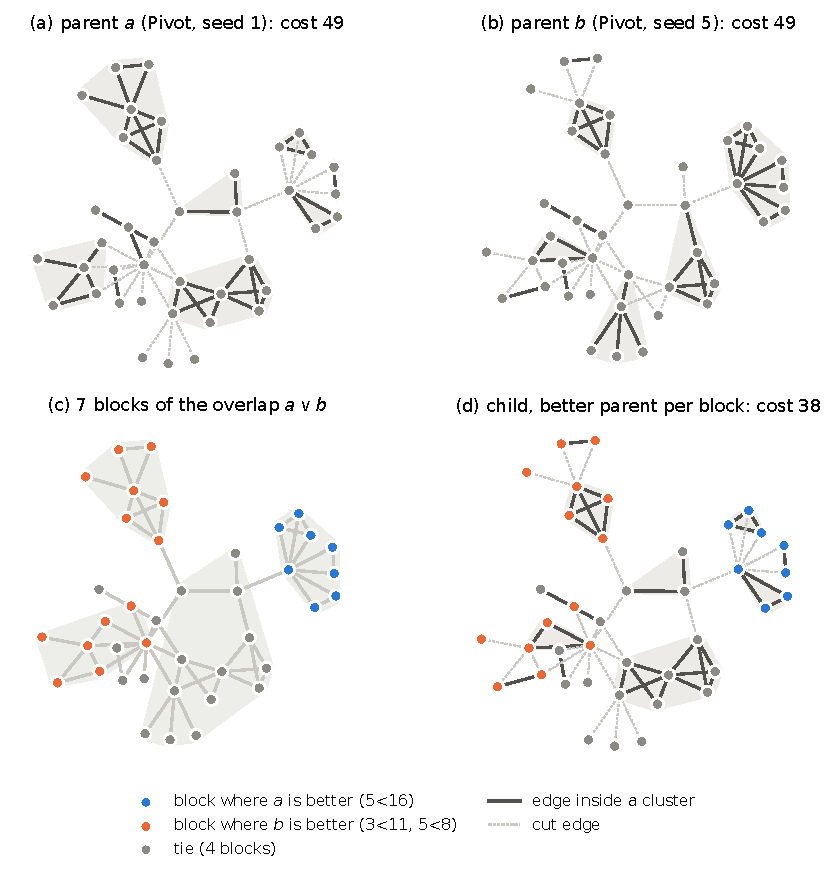
\includegraphics[width=0.88\textwidth]{figures/fig_crossover.pdf}
\caption{Partition crossover (Theorem~\ref{thm:px}) computed by the released
code.  (a), (b): two Pivot clusterings of the neighbourhood of
Figure~\ref{fig:support}, both of cost 49; shaded regions are clusters.
(c): the connected components of the overlap graph $H$ split the vertices into
seven blocks, and on each block the two parents can be compared on their own.
(d): taking the better parent on every block gives a clustering of cost 38,
better than both parents.}\label{fig:crossover}
\end{figure}

\begin{theorem}[partition crossover]\label{thm:px}
Let the cost of a clustering be any sum of pair terms that depend only on
whether the two vertices of the pair share a cluster (this covers $\cost$ and
the weighted cost~\eqref{eq:wcost}).  Let $a$ and $b$ be clusterings and let
$H$ be the bipartite graph whose nodes
are the clusters of $a$ and of $b$, with an edge between $A\in a$ and $B\in b$
whenever $A\cap B\ne\emptyset$.  Each connected component of $H$ covers a
vertex set $X$, the \emph{block}, which is a union of clusters of $a$ and also
a union of clusters of $b$.  For a clustering $c$ let $\cost_X(c)$ count the
mistakes on the pairs inside $X$.  Choose, independently in every block, the
clusters of $b$ if $\cost_X(b)<\cost_X(a)$ and those of $a$ otherwise.  The
resulting clustering $\chi$ satisfies
\[
\cost(\chi)=\cost(a)-\sum_X\max\bigl(0,\cost_X(a)-\cost_X(b)\bigr)
\le\min\bigl(\cost(a),\cost(b)\bigr).
\]
\end{theorem}
\begin{proof}
A pair $u,v$ in different blocks is separated by $a$, by $b$ and by $\chi$,
because each of their clusters lies inside one block.  It therefore
contributes the same amount to all three costs.  A pair inside a block $X$ is
treated by $\chi$ exactly as by the parent chosen for $X$.  Summing over the
pairs gives the equality.  Every term of the sum is non-negative, and
exchanging the roles of $a$ and $b$ gives the bound by $\cost(b)$.
\end{proof}

The blocks are the connected components of a bipartite graph with at most $n$
edges, and the block costs need one pass over $\Ep$.  Hence $\chi$ is computed in
$O(n+m)$ time.  The blocks form the join $a\vee b$ of the two partitions in the partition
lattice: the finest partition whose parts are unions of clusters of $a$ and
also of $b$.  It is the finest partition for which every block-wise choice
between the parents yields each parent as one of the choices and leaves the
pairs between blocks separated in both.  Decomposing two parents into independent components and taking the better
parent in each is the partition crossover of
\citet{WhitleyHH09gpx,WhitleyHH10hybrid,TinosWO20gpx2} for tours and of
\citet{TinosWC15px} for pseudo-Boolean functions; recombination through the
overlap of groups is common in grouping genetic
algorithms~\citep{Falkenauer98grouping,GalinierH99coloring}, memetic graph
partitioning and clustering~\citep{SandersS12kaffpae,BiedermannHSS18memetic}
and ensemble clustering~\citep{OvelgonneG13ensemble}, and fusion
moves~\citep{BeierHK15fusion} combine proposals optimally within a restricted
space.  Theorem~\ref{thm:px} combines \emph{any} two clusterings, including
clusterings produced by different solvers.  On our graphs, two independent runs typically differ in thousands of
blocks, most of them ties, and each run wins some of the others.

\subsection{Annealing moves}

The search moves nodes of the contracted instance.  Let $S_X=\sum_{K\in X}s_K$
be the size of a cluster $X$ and $w(K,X)=\sum_{L\in X\setminus\{K\}}w_{KL}$.
Moving a node $K$ of size $s$ from its cluster $A$ to a cluster $B$ changes
$\cost_w$ by
\begin{equation}\label{eq:move}
\delta=s\,(S_B-S_A+s)+2\,\bigl(w(K,A)-w(K,B)\bigr).
\end{equation}
Exchanging $K\in A$ with $L\in B$ changes it by the sum of two such terms,
where the second one uses $S_A-s_K$, $S_B+s_K$, $w(L,B)+w_{KL}$ and
$w(L,A)-w_{KL}$.  Both are evaluated in $O(\deg K+\deg L)$ time.  The
simulated annealing~\citep{KirkpatrickGV83} proposes the move to the cluster
of a random neighbour, the best move, or a move to a new cluster, and accepts
with the Metropolis rule under a geometric cooling schedule.  It records the
best state with an undo journal, so a new best state costs $O(1)$ instead of
a copy of the labelling.  This alone made the annealing $7.3$ times faster on
\texttt{com-Amazon}.

\paragraph{Region-wise acceptance.}  Theorem~\ref{thm:px} turns annealing into
an iterated local search with a decomposed acceptance test.  From the current
clustering $x$ we anneal a copy, starting at a raised temperature, down to its
final state $y$, and set $x\gets\chi(x,y)$.  Every block in which $y$ improved
on $x$ is kept, even if $y$ is worse overall, and the cost of $x$ never
increases.

\paragraph{Localized annealing with rollback.}  A step grows a region of at
most $30$ nodes by breadth-first search around a centre, anneals only the
nodes of the region from a high to a low temperature, finishes with greedy best
moves, and undoes all moves if their total change is positive.  The undo is
exact: moves are reversed in LIFO order together with the free list of
cluster labels.  Half of the centres are drawn with probability proportional to
the degree.  Comparing our solutions with those of KaPoCE block by block showed
why: the blocks in which KaPoCE was better all contained a vertex of high
degree.

\subsection{The memetic search}

\begin{algorithm}[t]
\caption{PXMem$(G^+,T)$}\label{alg:pxmem}
\begin{algorithmic}[1]
\State contract the critical cliques
\For{$i=1,\dots,4$}
  \State $p_i\gets\textsc{Pivot}(G^+)$; $f_i\gets$ one round of \textsc{IteratedFlip}$(p_i)$
  \State $x_i\gets$ the cheaper of $p_i$ and $f_i$ on the contracted nodes; anneal $x_i$
\EndFor
\While{time remains}
  \State choose an operator by an $\varepsilon$-greedy bandit on the recent gain per second
  \State \textbf{crossover:} parents $a,b$ by binary tournaments; $z\gets\chi(a,b)$;
  \Statex \hspace{\algorithmicindent} contract the blocks common to $a$ and $b$ and run a multilevel local search from $z$;
  \Statex \hspace{\algorithmicindent} anneal on the nodes where $a$ and $b$ disagree; accept region-wise; crowding replacement
  \State \textbf{PX-annealing step} on a member (temperature chosen by a second bandit)
  \State \textbf{localized annealing} with rollback on a member
\EndWhile
\State \Return the cheapest member, expanded to $V$
\end{algorithmic}
\end{algorithm}

Algorithm~\ref{alg:pxmem} keeps a population of four clusterings.  A crossover
child enters the population only by replacing a member that is not cheaper,
preferring the most similar members (crowding); the other two operators
replace a member only if they improve it.  Contracting the blocks common to
both parents and continuing with a multilevel search from the recombined
clustering follows the recombination of memetic graph partitioners and
clusterers~\citep{SandersS12kaffpae,BiedermannHSS18memetic,hausberger2025scc}.  The flipping round of line~3 costs a few
full local-search passes whatever its time limit; with budgets below
\SI{300}{s} the seeds are therefore Pivot clusterings only, and no further seed
is generated once half of the budget is used.

\begin{theorem}\label{thm:pxmem}
Let $\mathcal C$ be the output of Algorithm~\ref{alg:pxmem} and $p_1$ the first
Pivot clustering.  Then $\cost(\mathcal C)\le\cost(p_1)$ for every outcome of
the random choices, and hence $\mathbb E[\cost(\mathcal C)]\le3\,\OPT$.  Together
with a lower bound $\LB$ from Section~\ref{sec:dual},
$\cost(\mathcal C)/\lceil\LB\rceil$ bounds the ratio achieved on the instance.
\end{theorem}
The guarantee is inherited from the Pivot seed, as for any procedure that
starts from a Pivot clustering and never makes its best solution worse; we state
it because every operator of the search must respect it, and this is what the
formal development checks.

\begin{proof}
The seed $x_1$ costs at most $\cost(p_1)$: Pivot does not separate twins, so its
contraction preserves its cost, and $x_1$ is the cheaper of the two
candidates.  The annealing returns the cheapest state of a trajectory that
starts at its input; region-wise acceptance does not increase the cost by
Theorem~\ref{thm:px}; the localized annealing keeps a step only if its total
change is non-positive; and every replacement is by a clustering that is not
more expensive than the member it replaces.  By induction over the
replacements, some member always costs at most $\cost(x_1)$, so the cheapest
final member costs at most $\cost(p_1)$.  Taking expectations and applying the
Pivot guarantee~\citep{AilonCN08} gives the second claim.  The last claim is
Theorem~\ref{thm:anytime}(a).
\end{proof}


\subsection{Comparison with KaPoCE}\label{sec:exp-h2h}

\paragraph{Protocol.}  PXMem and KaPoCE are compared under a
protocol that was fixed before the runs
(\texttt{experiments/heldout.md}).  On one machine, the two solvers run one
after the other in an order drawn from a hash of (graph, seed), each on the
same logical core while the machine is otherwise idle.  Both read the same
PACE-format text file inside their measured time.  KaPoCE's only changes are
a seed and its two internal time limits, set to $\tfrac{590}{600}T$ and
$\tfrac{90}{600}T$ (the ratio of its PACE configuration); it is stopped with
SIGTERM at $T$ and its output is validated.  PXMem is scored at KaPoCE's
elapsed wall-clock time, read from its improvement history, so the
comparison is at equal elapsed time; its value at $T$ is also recorded.
Invalid KaPoCE output counts as a PXMem win, as in PACE, and is reported
separately.  Budgets are $T=\SI{600}{s}$ (primary), \SI{150}{s} and
\SI{60}{s}, with ten seeds on each held-out SNAP graph and one run on each
PACE heuristic instance at \SI{600}{s}.

\paragraph{Statistics.}  The unit of inference is the graph.  For each graph
we take the median over seeds of the relative difference
$(\cost_{\mathrm{PXMem}}-\cost_{\mathrm{KaPoCE}})/\cost_{\mathrm{KaPoCE}}$ and
apply the two-sided Wilcoxon signed-rank test~\cite{Wilcoxon45} and the sign
test to the twelve medians.  Per graph we report the exact sign test over
seeds with Holm's correction~\cite{Holm79} over graphs, noting that with ten
seeds only a 10:0 split can be significant, and the Hodges--Lehmann
estimate~\cite{HodgesL63} of the paired difference with its exact confidence
interval.  We do not claim equivalence from non-significance.  Performance
profiles~\cite{DolanM02profiles} summarise the PACE heuristic track.


\begin{table}[!tbp]
\centering
\caption{PXMem against KaPoCE on the twelve held-out SNAP graphs,
$T=\SI{600}{s}$ (primary budget), ten seeds per graph.  W/T/L: runs in
which PXMem is better, equal, worse.  median, HL: median and Hodges--Lehmann
estimate of $(\cost_{\mathrm{PXMem}}-\cost_{\mathrm{KaPoCE}})/
\cost_{\mathrm{KaPoCE}}$ in percent, negative when PXMem is better, with the
exact $95\%$ confidence interval; $p$: exact sign test over the seeds;
$p_{\mathrm{Holm}}$: Holm-adjusted over the twelve graphs.  Last row: the
pre-registered tests over the twelve graph medians.}
\label{tab:h2h-600}
\footnotesize
\setlength{\tabcolsep}{4pt}
\pending{}

\end{table}

\begin{table}[!tbp]
\centering
\caption{As Table~\ref{tab:h2h-600}, $T=\SI{150}{s}$.}
\label{tab:h2h-150}
\footnotesize
\setlength{\tabcolsep}{4pt}
\begin{tabular}{lrcrlrr}
\toprule
graph & runs & W/T/L & median (\%) & HL (\%) [95\% CI] & $p$ & $p_{\mathrm{Holm}}$ \\
\midrule
\texttt{email-Eu-core} & 6 & 0/5/1 & $+0.000$ & $+0.000$ [$+0.000$, $+0.008$] & 1.000 & 1.000 \\
\texttt{facebook} & 6 & 0/6/0 & $+0.000$ & $+0.000$ [$+0.000$, $+0.000$] & 1.000 & 1.000 \\
\texttt{wiki-Vote} & 6 & 5/0/1 & $-0.008$ & $-0.007$ [$-0.016$, $+0.026$] & 0.219 & 1.000 \\
\texttt{cit-HepTh} & 5 & 4/0/1 & $-0.009$ & -- & 0.375 & 1.000 \\
\texttt{cit-HepPh} & 6 & 3/0/3 & $-0.000$ & $-0.000$ [$-0.021$, $+0.039$] & 1.000 & 1.000 \\
\texttt{p2p-Gnutella31} & 6 & 0/4/2 & $+0.000$ & $+0.000$ [$+0.000$, $+0.001$] & 0.500 & 1.000 \\
\texttt{soc-Slashdot0902} & 6 & 0/0/6 & $+0.006$ & $+0.007$ [$+0.004$, $+0.010$] & 0.031 & 0.375 \\
\texttt{loc-Gowalla} & 5 & 0/0/5 & $+0.008$ & -- & 0.062 & 0.688 \\
\texttt{email-EuAll} & 5 & 5/0/0 & $-0.011$ & -- & 0.062 & 0.688 \\
\texttt{amazon0302} & 5 & 0/0/5 & $+0.008$ & -- & 0.062 & 0.688 \\
\texttt{web-NotreDame} & 5 & 0/0/5 & $+0.022$ & -- & 0.062 & 0.688 \\
\texttt{roadNet-PA} & 4 & 0/0/4 & $+0.507$ & -- & 0.125 & 0.875 \\
\midrule
\multicolumn{7}{l}{graph medians: 4 better, 3 equal, 5 worse; Wilcoxon $p=0.652$, sign test $p=1.000$} \\
\bottomrule
\end{tabular}

\end{table}

\begin{table}[!tbp]
\centering
\caption{As Table~\ref{tab:h2h-600}, $T=\SI{60}{s}$.}
\label{tab:h2h-60}
\footnotesize
\setlength{\tabcolsep}{4pt}
\pending{}

\end{table}

\paragraph{Primary budget.}  At \SI{600}{s} (Table~\ref{tab:h2h-600},
\numHHSixRuns{} paired runs) the graph medians favour PXMem on
\numHHSixBetter{} graphs and KaPoCE on \numHHSixWorse{}, with
\numHHSixEqual{} ties.  Neither pre-registered test rejects equality of the
two solvers (Wilcoxon $p=\numHHSixWilcoxon$, sign test
$p=\numHHSixSign$).  After Holm's correction PXMem is better on
\texttt{loc-Gowalla} and KaPoCE on \texttt{amazon0302} and
\texttt{roadNet-PA}; PXMem wins nine of ten seeds on \texttt{wiki-Vote},
\texttt{cit-HepTh} and \texttt{cit-HepPh}, which is not significant after the
correction.  All differences are small: the largest graph median is
\numHHSixMaxAbs{}, and on the held-out graphs with a certificate the
certified gap of the best solution is at least \numSnapGapMinHeld{}
(Table~\ref{tab:snap-bounds}).  The certificates therefore cannot separate
the two solvers, and neither solver is shown to be near-optimal on these
graphs beyond what Table~\ref{tab:snap-bounds} certifies.  KaPoCE returned a
valid solution in every run (\numHHSixForfeitK{} forfeits).  Scoring PXMem at
$T$ instead of at KaPoCE's elapsed time gives \numHHSixAtTBetter{} better and
\numHHSixAtTWorse{} worse graph medians (Wilcoxon $p=\numHHSixAtTWilcoxon$).
Many per-seed differences are zero or tied on some graphs
(\texttt{email-Eu-core}, \texttt{facebook}, \texttt{p2p-Gnutella31}); there
the Hodges--Lehmann interval degenerates and its coverage is not exact, and
zero graph medians are dropped from the Wilcoxon test, which the analysis
plan did not specify.  We do not claim that the two solvers are
equivalent: the study was not designed as an equivalence test.

\paragraph{Shorter budgets.}  KaPoCE did not stop by itself and was
terminated by SIGTERM in \numHHSixSigterm{}, \numHHOneFiftySigterm{} and
\numHHSixtySigterm{} of the 120 runs at \SI{600}{s}, \SI{150}{s} and
\SI{60}{s}; it then writes its best solution, which can take some seconds,
while PXMem is scored at KaPoCE's elapsed time.  This favours KaPoCE.  At
\SI{150}{s} (Table~\ref{tab:h2h-150}) the picture is similar (\numHHOneFiftyBetter{} better, \numHHOneFiftyEqual{}
equal, \numHHOneFiftyWorse{} worse; Wilcoxon $p=\numHHOneFiftyWilcoxon$),
with larger losses of PXMem on the largest graphs, up to
\numHHOneFiftyMaxAbs{} on \texttt{roadNet-PA}.  At \SI{60}{s}
(Table~\ref{tab:h2h-60}) KaPoCE is better on \numHHSixtyWorse{} of the
\numHHSixtyGraphs{} graph medians (Wilcoxon $p=\numHHSixtyWilcoxon$).  PXMem is
a population method, and a short budget leaves few recombinations on graphs
with $10^5$ vertices or more; we did not analyse this further.  PXMem is thus
not a replacement for KaPoCE at short budgets, and at the primary budget the
two are not distinguishable by our tests.

\paragraph{PACE heuristic track.}  On the 200 instances of the PACE~2021
heuristic track, one run per instance at \SI{600}{s} under the same protocol,
the instance is the unit.  The \numPDn{} instances that coincide with
development graphs are reported separately (Table~\ref{tab:pace-heur}).  On
the other \numPHn{} instances PXMem is better on \numPHBetter{}, equal on
\numPHEqual{} and worse on \numPHWorse{} (Wilcoxon $p=\numPHWilcoxon$, sign
test $p=\numPHSign$); KaPoCE returned no valid solution on
\numPHKapoceInvalid{} instances, which count as PXMem wins as in PACE.
The counts hide the sizes of the differences: summed over the \numPHn{}
instances the costs favour KaPoCE by 5185, and the eleven instances with
$10^5$ vertices or more contribute 5344 of this (PXMem better on six of
them, worse on five).
PXMem records its first solution only after its initialisation; on
\numPHNoSolution{} small instance KaPoCE stopped before that, and it
counts as a KaPoCE win under the protocol.
Figure~\ref{fig:profile} shows the performance profile.

\begin{table}[!tbp]
\centering
\caption{PACE~2021 heuristic track, $T=\SI{600}{s}$, one run per instance:
PXMem against KaPoCE by instance size.  W/T/L: instances on which PXMem is
better, equal, worse; $\sum$: total difference of the costs; median: of the
relative differences in percent.}
\label{tab:pace-heur}
\footnotesize
\begin{tabular}{l}
\pending{} (54 of 200 runs done)
\end{tabular}

\end{table}

\begin{figure}[!tbp]
\centering
\IfFileExists{figures/profile_pace_heur.pdf}{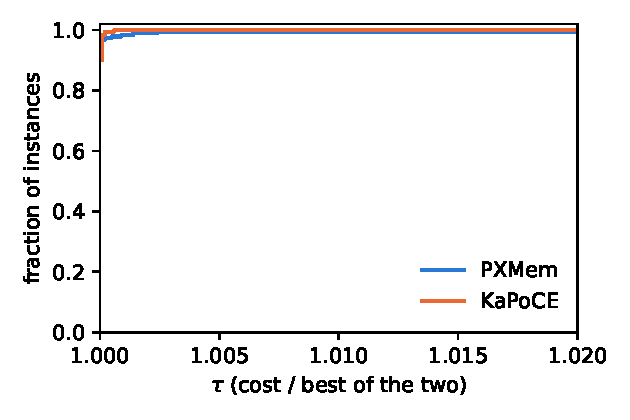
\includegraphics[width=0.6\textwidth]{figures/profile_pace_heur.pdf}}{\pending{}}
\caption{Performance profile~\cite{DolanM02profiles} on the PACE heuristic
track without the development twins: fraction of instances on which a
solver's cost is within a factor $\tau$ of the better of the two.}
\label{fig:profile}
\end{figure}


\section{Development log}\label{app:devlog}

This appendix records which data informed which decision, so that the
reader can judge which results are out of sample.

\begin{itemize}
\item \emph{Development data.}  The fifteen SNAP graphs of
Table~\ref{tab:instances} marked ``dev'' and the 200 PACE~2021 exact-track
instances.  All parameters of the bound (block size $2500$, $|H|\le8$ for local
subgraph rows, ruin regions of about $12$ vertices, a target of half of the
remaining budget for the bound), of the LNS ($|B|\le60$) and of PXMem (population $4$, regions of at
most $30$ nodes, bandit settings, the degree bias of the region centres)
were chosen by looking at runs on these instances.  Several PXMem components
were added after inspecting where KaPoCE's solutions were better than ours on
development graphs (Section~\ref{sec:primal}).
\item \emph{Earlier comparisons.}  A head-to-head comparison with KaPoCE on
the development graphs and on the PACE heuristic track was carried out before
the held-out set was fixed.  Its raw results remain in the repository; it is
not the basis of any claim in this paper, because the same graphs were used
for tuning and because it measured the two solvers asymmetrically (KaPoCE's
time included reading the input, PXMem's did not, and the order was fixed).
\item \emph{Machines.}  Earlier runs of the PACE exact track on a 4-core
workstation with four runs in parallel, also with checked certificates,
proved optimality on 111 of the 173 solved instances.  All numbers in this
paper are from the runs on the Colab machines described in
Section~\ref{sec:exp-setup}, which give \numPaceOptOurs{}; we report the
latter because the other bounds of Table~\ref{tab:pace-bounds} were computed
on the same machines and because their certificates are the archived ones.
\item \emph{Held-out data.}  The twelve SNAP graphs marked ``held-out'' in
Table~\ref{tab:instances} and the analysis plan of
Section~\ref{sec:exp-setup} were fixed and committed to the repository
(\texttt{experiments/heldout.md}) before any bound was computed on them and
before any run of the protocol.  The plan states that no earlier run of
either solver on them existed; this is not correct.  Seven of the held-out
graphs are PACE heuristic-track instances, and all 200 heuristic-track
instances had been run once with both solvers in the earlier comparison
above.  That comparison was made after the last change to the solver code
(the code has not changed since), and it informed no parameter, but its
results were known when the held-out set was chosen.  The ten
heuristic-track instances that coincide with development graphs are
reported separately; the other 190 were not used for tuning, but they are not
held out in the strict sense.
\item \emph{Gap-guided search.}  We did not evaluate the gap-guided choice of
blocks and LNS neighbourhoods separately in the final experiments.  In the
development runs (\texttt{results/ablation\_lb.csv}, five development graphs,
4-core workstation, \SI{300}{s}), gap-guided blocks after the METIS sweeps
changed the bound by $-0.004\%$ to $+0.03\%$; the same runs gave larger
bounds with block LPs after a packing than with a packing alone on all five
graphs.
\item \emph{Headline bound.}  The decision to report the largest of the
CertiFlip bound, the separate star-packing bound and the long packing
followed by block LPs on the SNAP graphs was taken after the packing runs
were complete, and the last procedure and the packing runs on the graphs
above the support threshold were added after the second round of review;
all three are valid, and all are reported per graph.  The result files of
the long-packing runs record the commit of the code package they were
started from, which predates the script mode that ran them; the solver
code was not changed between the two.
\item \emph{Star local search.}  The star local search was written after all
other results in this paper were known, when a rerun of the lower-bound
program of the branch-and-bound had shown that its root packing was far
stronger than our ruin-and-recreate packing on the same rows.  It follows the
heuristic of that program; the program's code was read to understand the
heuristic, and none of it was copied (the solver is GPL-licensed, ours is
BSD).  While testing it on nine PACE exact instances we found and fixed one
error (trying and undoing a leaf extension invalidated the remaining
candidates of that star), and before the final runs it was tried for 60 to
\SI{120}{s} on nine SNAP graphs, seven of them held out (\texttt{facebook},
\texttt{email-Eu-core}, \texttt{wiki-Vote}, \texttt{cit-HepPh},
\texttt{amazon0302}, \texttt{roadNet-PA}, \texttt{loc-Gowalla}) and two
development graphs (\texttt{ca-HepPh}, \texttt{com-DBLP}); nothing was changed
after these trials.  Its parameters (at most five unimproved rounds per
improving one, probability $0.8$ for the plateau move, 16 candidates per
freed pair) are those of the branch-and-bound or were not tuned; the time
limits, \SI{60}{s} on PACE and \SI{600}{s} on SNAP, are those of the CertiFlip
runs.  All reported runs are from one version of its code, except the leaf
cap on two graphs, which was added after their first runs had been killed.
Its runs are therefore not out of sample in the sense of the held-out
protocol, which was fixed for the head-to-head comparison.
\end{itemize}


\bibliographystyle{plainnat}
\bibliography{refs}

\end{document}
